\documentclass[aspectratio=169]{beamer}
\usepackage[utf8]{inputenc}
\usepackage{tikz} % for QR code overlay

% code snippets
\usepackage{minted}
\newmintedfile[dockercode]{dockerfile}{
  % bgcolor=mintedbackground,
  fontfamily=tt,
  linenos=true,
  numberblanklines=true,
  numbersep=5pt,
  gobble=0,
  frame=leftline,
  framerule=0.4pt,
  framesep=2mm,
  funcnamehighlighting=true,
  tabsize=4,
  obeytabs=false,
  mathescape=false
  samepage=false, %with this setting you can force the list to appear on the same page
  showspaces=false,
  showtabs =false,
  texcl=false,
}
\newminted[bashcode]{bash}{
  % bgcolor=mintedbackground,
  fontfamily=tt,
  linenos=true,
  numberblanklines=true,
  numbersep=5pt,
  gobble=0,
  frame=leftline,
  framerule=0.4pt,
  framesep=2mm,
  funcnamehighlighting=true,
  tabsize=4,
  obeytabs=false,
  mathescape=false
  samepage=false, %with this setting you can force the list to appear on the same page
  showspaces=false,
  showtabs =false,
  texcl=false,
}

% biblatex (requires biber; sudo pacman -S biber)
\usepackage[]{biblatex} % biblatex
\addbibresource{./content/bib/bib1.bib}
\addbibresource{./content/bib/bib2.bib}
\addbibresource{./content/bib/throwaway.bib}

\usepackage{graphicx}
\graphicspath{ {./content/img/} }

\usetheme{Boadilla}
\usecolortheme{rose}
% \beamerdefaultoverlayspecification{<+->} % this will turn it into slides

\title{Privacy-Preserving Encrypted Deep Learning}
\subtitle{Fully Homomorphic Encryption}
\author{George Onoufriou\\University of Lincoln}
\date{\today}

\begin{document}

\addtobeamertemplate{frametitle}{}{%
\begin{tikzpicture}[remember picture,overlay]
\node[anchor=north east,yshift=2pt] at (current page.north east) {
\includegraphics[height=1.5cm]{qrcode.png}};
\end{tikzpicture}}

  \frame{\titlepage}

  \begin{frame}
    \frametitle{About}
    \begin{columns}
      \begin{column}{0.5\textwidth}
        \begin{itemize}
          \item PhD Candidate Computer/ Data Science
          \item Privacy and Linux Enthusiast
        \end{itemize}
      \end{column}
      \begin{column}{0.5\textwidth}
        \begin{figure}[th!]
          \centering
          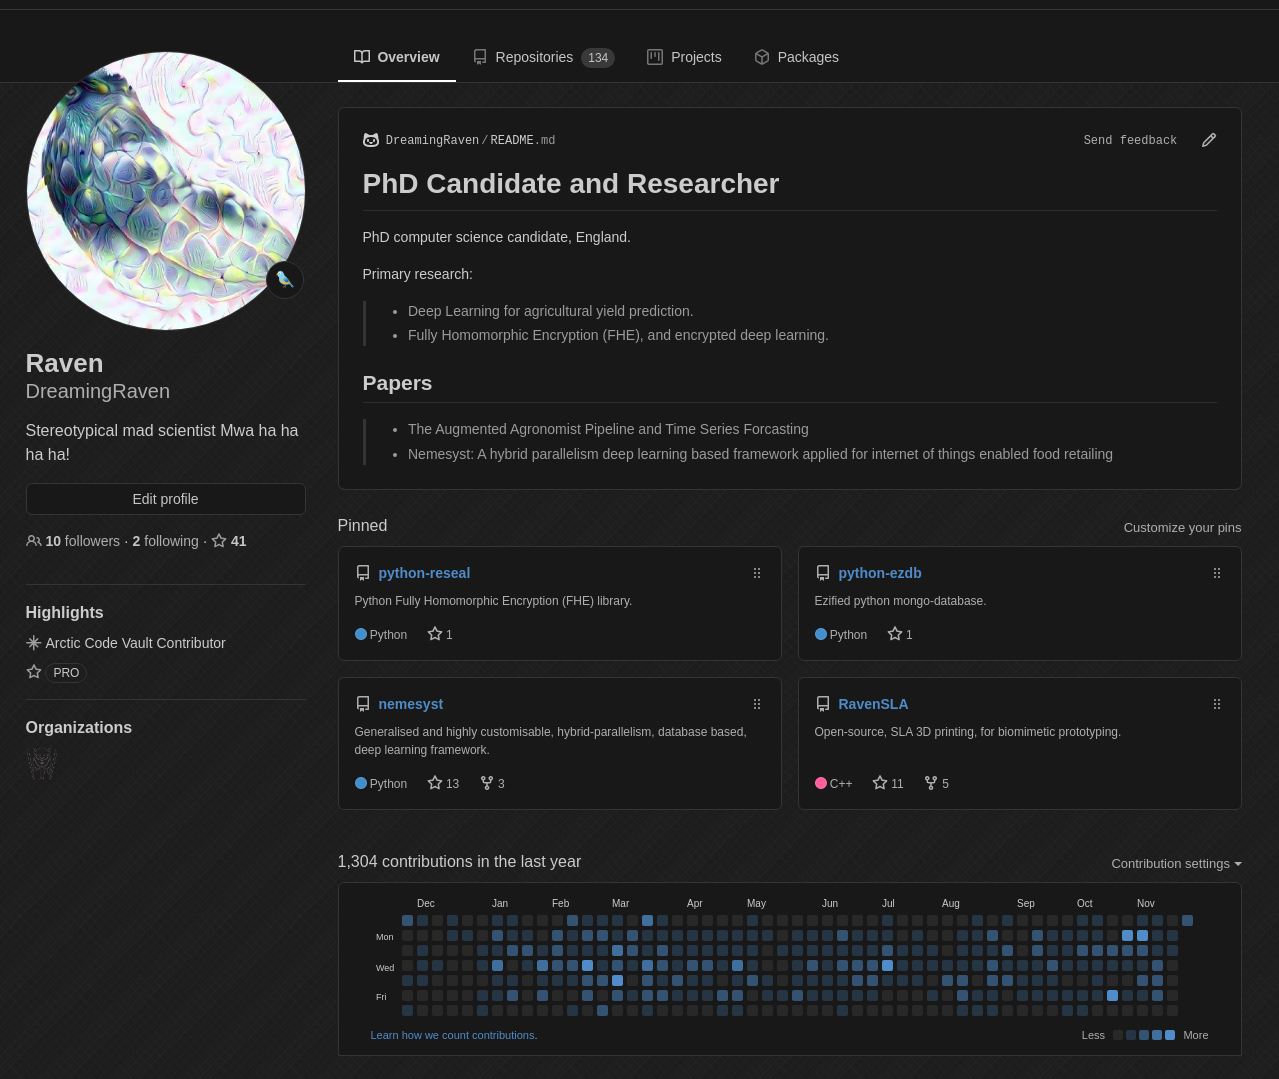
\includegraphics[width=0.8\textwidth]{gh.png}
          \caption{GitHub profile page where you can come to see my work and chat. \autocite{repository}}
          \label{fig:gh}
        \end{figure}
      \end{column}
    \end{columns}
  \end{frame}

  \begin{frame}
    \frametitle{My Work}
    \begin{columns}
      \begin{column}{0.5\textwidth}
        I work with:
        \begin{itemize}
          \item Deep Learning (subfield of Artificial Intelligence, and probably the coolest part of AI)
          \item Fully Homomorphic Encryption
        \end{itemize}
        Applied to:
        \begin{itemize}
          \item Agriculture; Predicting plant yield, in particular strawberries.
        \end{itemize}
      \end{column}
      \begin{column}{0.5\textwidth}
        \begin{figure}[th!]
          \centering
          \includegraphics[angle=-90,origin=c,width=0.55\textwidth]{wasp.jpg}
          \caption{Strawberry tabletop with a wasp having some lunch. \autocite{repository}}
          \label{fig:wasp}
        \end{figure}
      \end{column}

    \end{columns}
  \end{frame}

  \begin{frame}
    \frametitle{What is Artificial Intelligence}
    \begin{columns}
      \begin{column}{0.5\textwidth}
        \begin{itemize}
          \item T-800 coming for John Connor?
        \end{itemize}
      \end{column}
      \begin{column}{0.5\textwidth}
        \begin{figure}[th!]
          \centering
          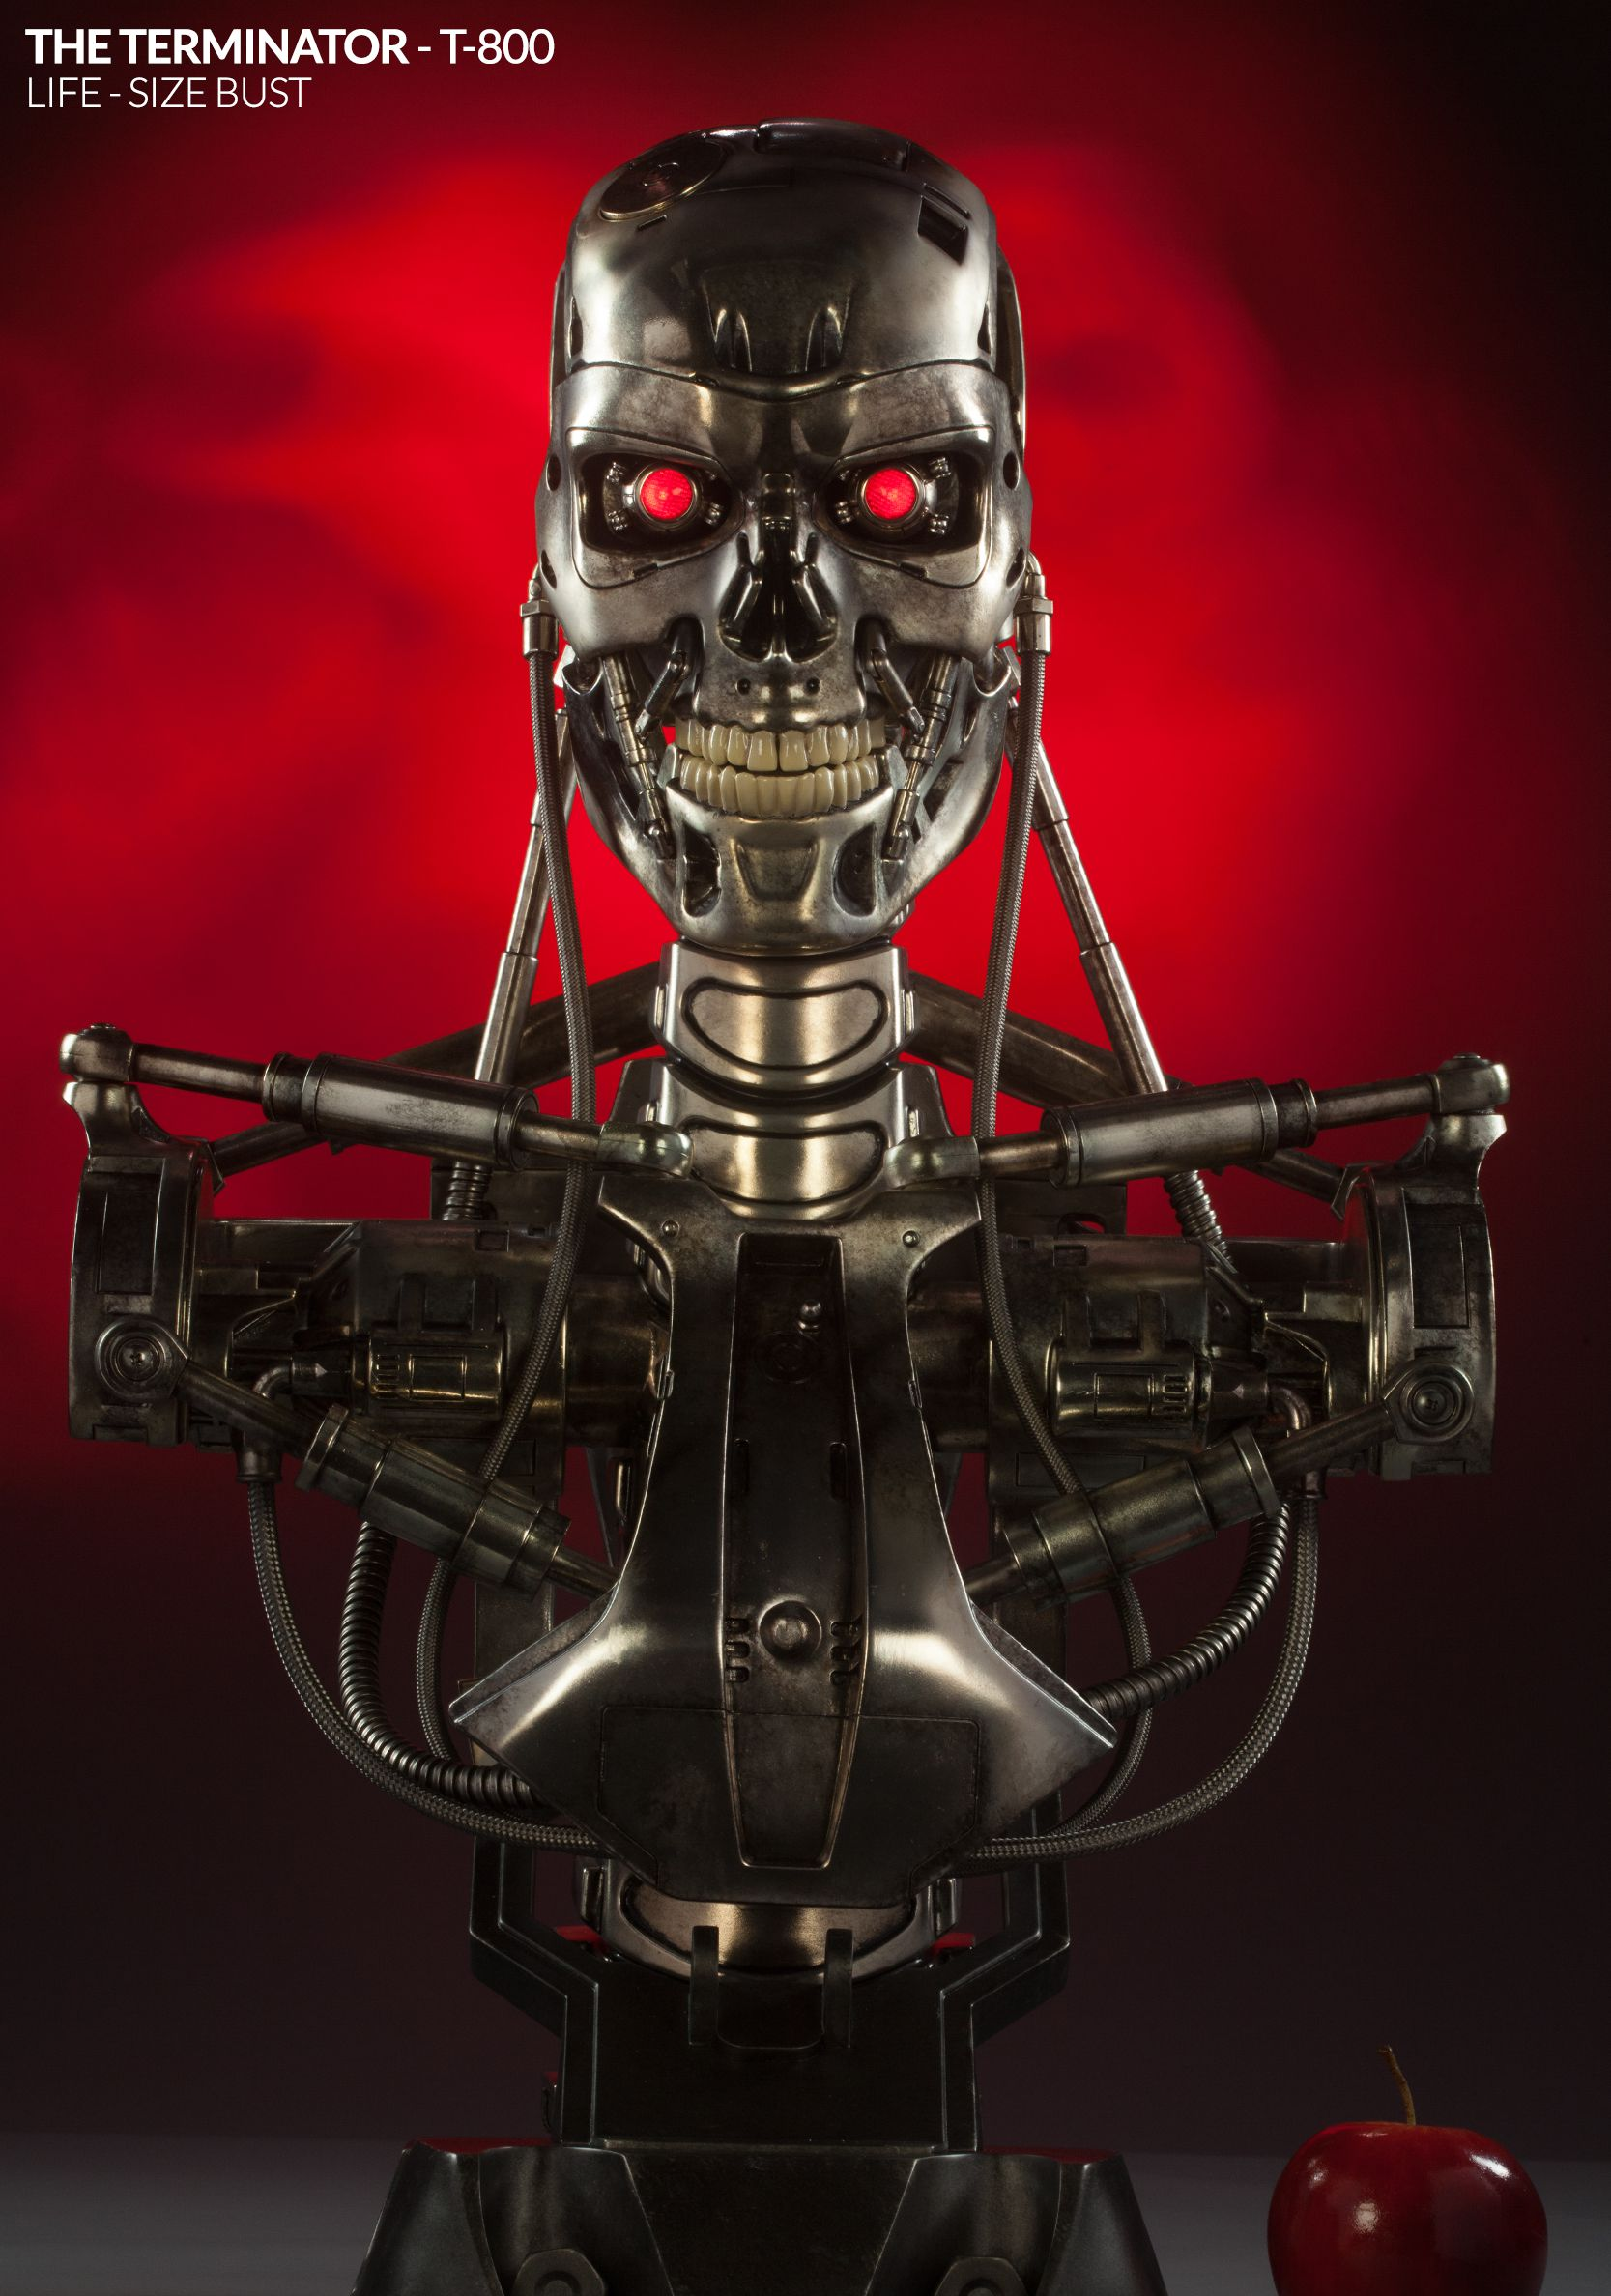
\includegraphics[width=0.5\textwidth]{t800.jpg}
          \caption{T-800, terminator bust from sideshow collectibles.}
          \label{fig:jim_carrey}
        \end{figure}
      \end{column}
    \end{columns}
  \end{frame}

  \begin{frame}
    \frametitle{What is Artificial Intelligence}
    \begin{columns}
      \begin{column}{0.5\textwidth}
        \begin{itemize}
          \item HAL9000?
        \end{itemize}
        Who in both the film and novel is capable of:
        \begin{itemize}
          \item Speech/ speech recognition, known as natural language processing (NLP)
          \item Facial recognition
          \item Lip reading
          \item Art appreciation
          \item Playing chess
        \end{itemize}
      \end{column}
      \begin{column}{0.5\textwidth}
        \begin{figure}[th!]
          \centering
          
\includegraphics[width=0.2\textwidth]{hal9000.pdf}
          \caption{HAL9000, Space Odyssey. Image by Grafiker61 \autocite{cc}}
          \label{fig:jim_carrey}
        \end{figure}
      \end{column}
    \end{columns}
  \end{frame}

  \begin{frame}
    \frametitle{What is Artificial Intelligence}
    \begin{columns}
      \begin{column}{0.5\textwidth}
        Who in both the film and novel is capable of:
        \begin{itemize}
          \item Speech/ speech recognition, known as natural language processing (NLP)
          \item Facial recognition
          \item Lip reading
          \item Art appreciation
          \item Playing chess $+$
        \end{itemize}
      \end{column}
      \begin{column}{0.5\textwidth}
        \begin{figure}[th!]
          \centering
          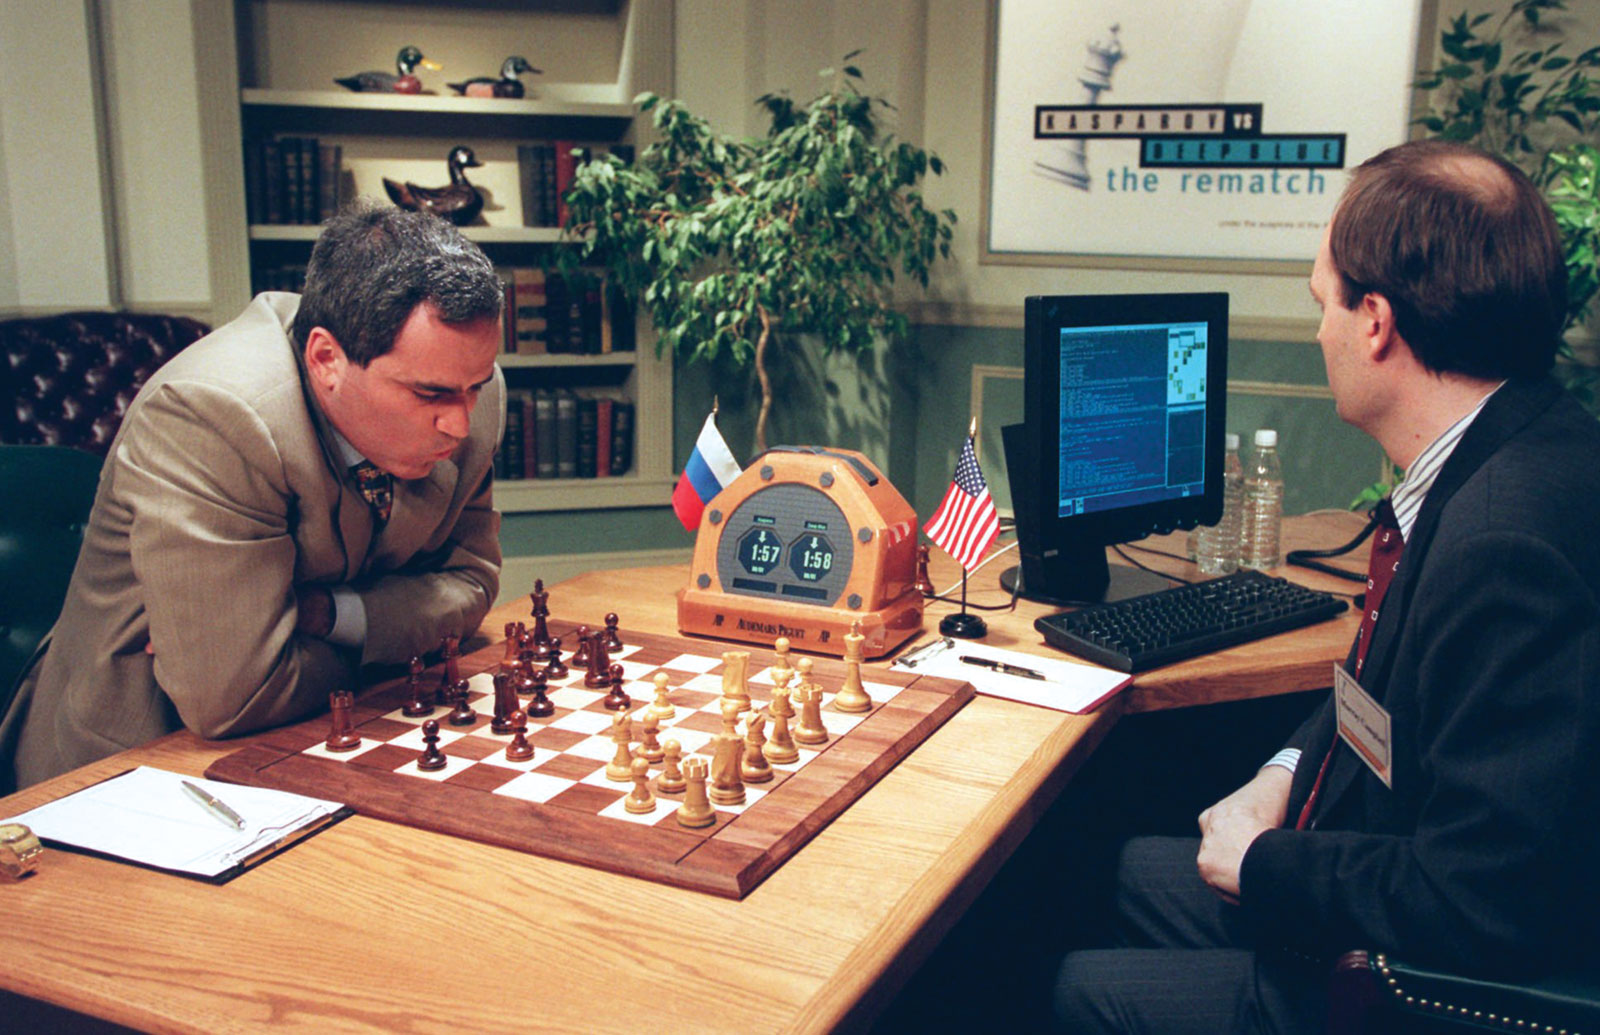
\includegraphics[width=1\textwidth]{deep-blue.jpg}
          \caption{Deep Blue rematch against world champion Garry Kasparov after beating him in 1996 (by Adam Nadel/AP Images)}
          \label{fig:jim_carrey}
        \end{figure}
      \end{column}
    \end{columns}
  \end{frame}

  \begin{frame}
    \frametitle{What is Artificial Intelligence}
    \begin{columns}
      \begin{column}{0.5\textwidth}
        Who in both the film and novel is capable of:
        \begin{itemize}
          \item Speech/ speech recognition, known as natural language processing (NLP) $+$
          \item Facial recognition
          \item Lip reading
          \item Art appreciation
          \item Playing chess
        \end{itemize}
      \end{column}
      \begin{column}{0.5\textwidth}
        \begin{figure}[th!]
          \centering
          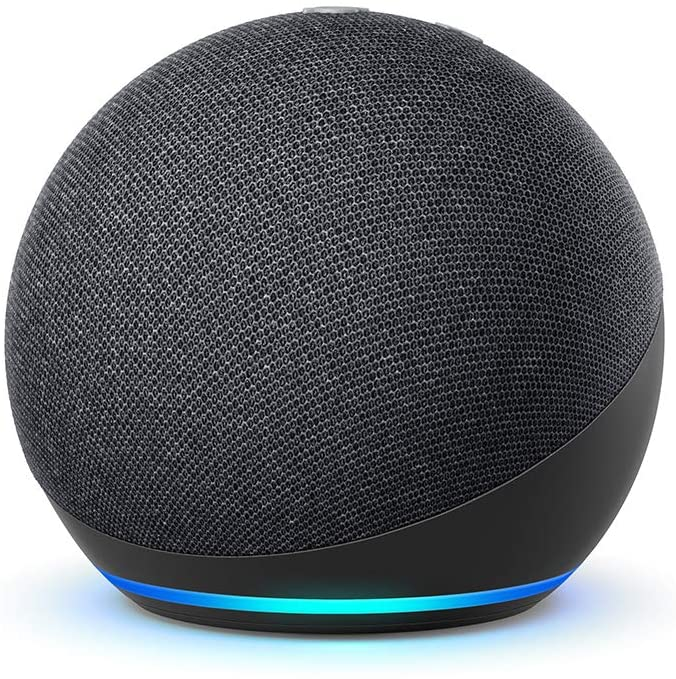
\includegraphics[width=0.5\textwidth]{alexa.jpg}
          \caption{Amazon Alexa, echo dot gen 4}
          \label{fig:jim_carrey}
        \end{figure}
      \end{column}
    \end{columns}
  \end{frame}

  \begin{frame}
    \frametitle{What is Artificial Intelligence}
    \begin{columns}
      \begin{column}{0.5\textwidth}
        Who in both the film and novel is capable of:
        \begin{itemize}
          \item Speech/ speech recognition, known as natural language processing (NLP)
          \item Facial recognition
          \item Lip reading
          \item Art appreciation $-$
          \item Playing chess
        \end{itemize}
      \end{column}
      \begin{column}{0.5\textwidth}
        \begin{figure}[th!]
          \centering
          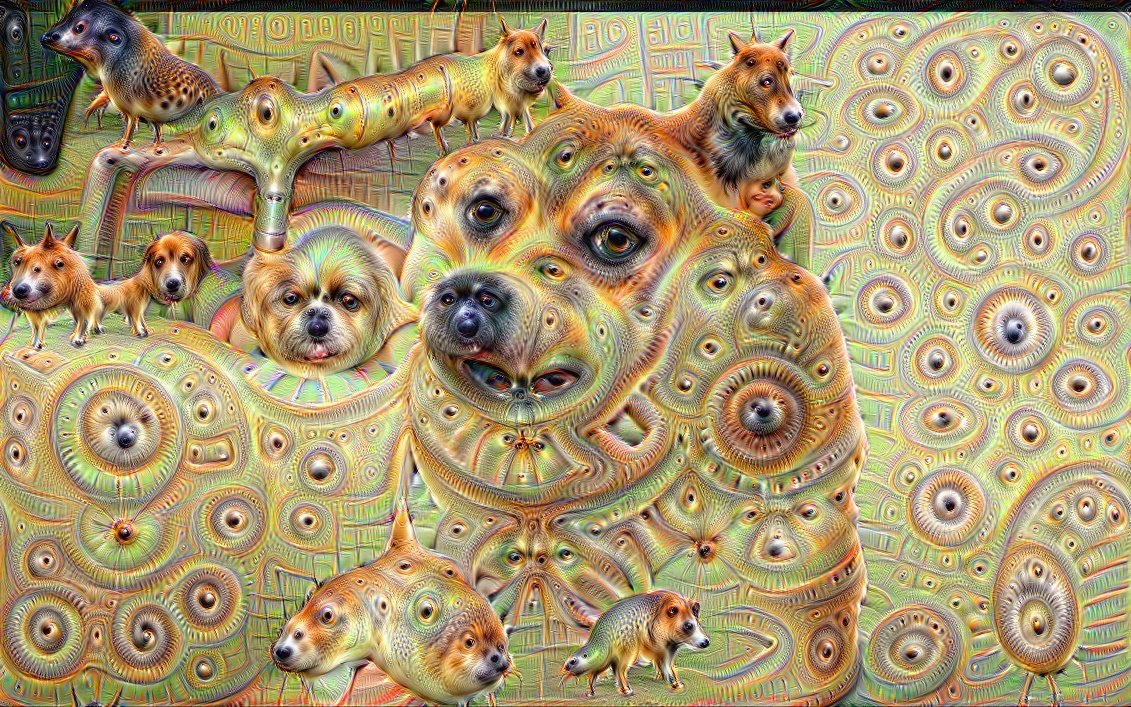
\includegraphics[width=0.9\textwidth]{deep-dream.jpg}
          \caption{Google Deep Dream Generator}
          \label{fig:jim_carrey}
        \end{figure}
      \end{column}
    \end{columns}
  \end{frame}

  \begin{frame}
    \frametitle{What is Artificial Intelligence}
    \begin{columns}
      \begin{column}{0.9\textwidth}
        \begin{figure}[th!]
          \centering
          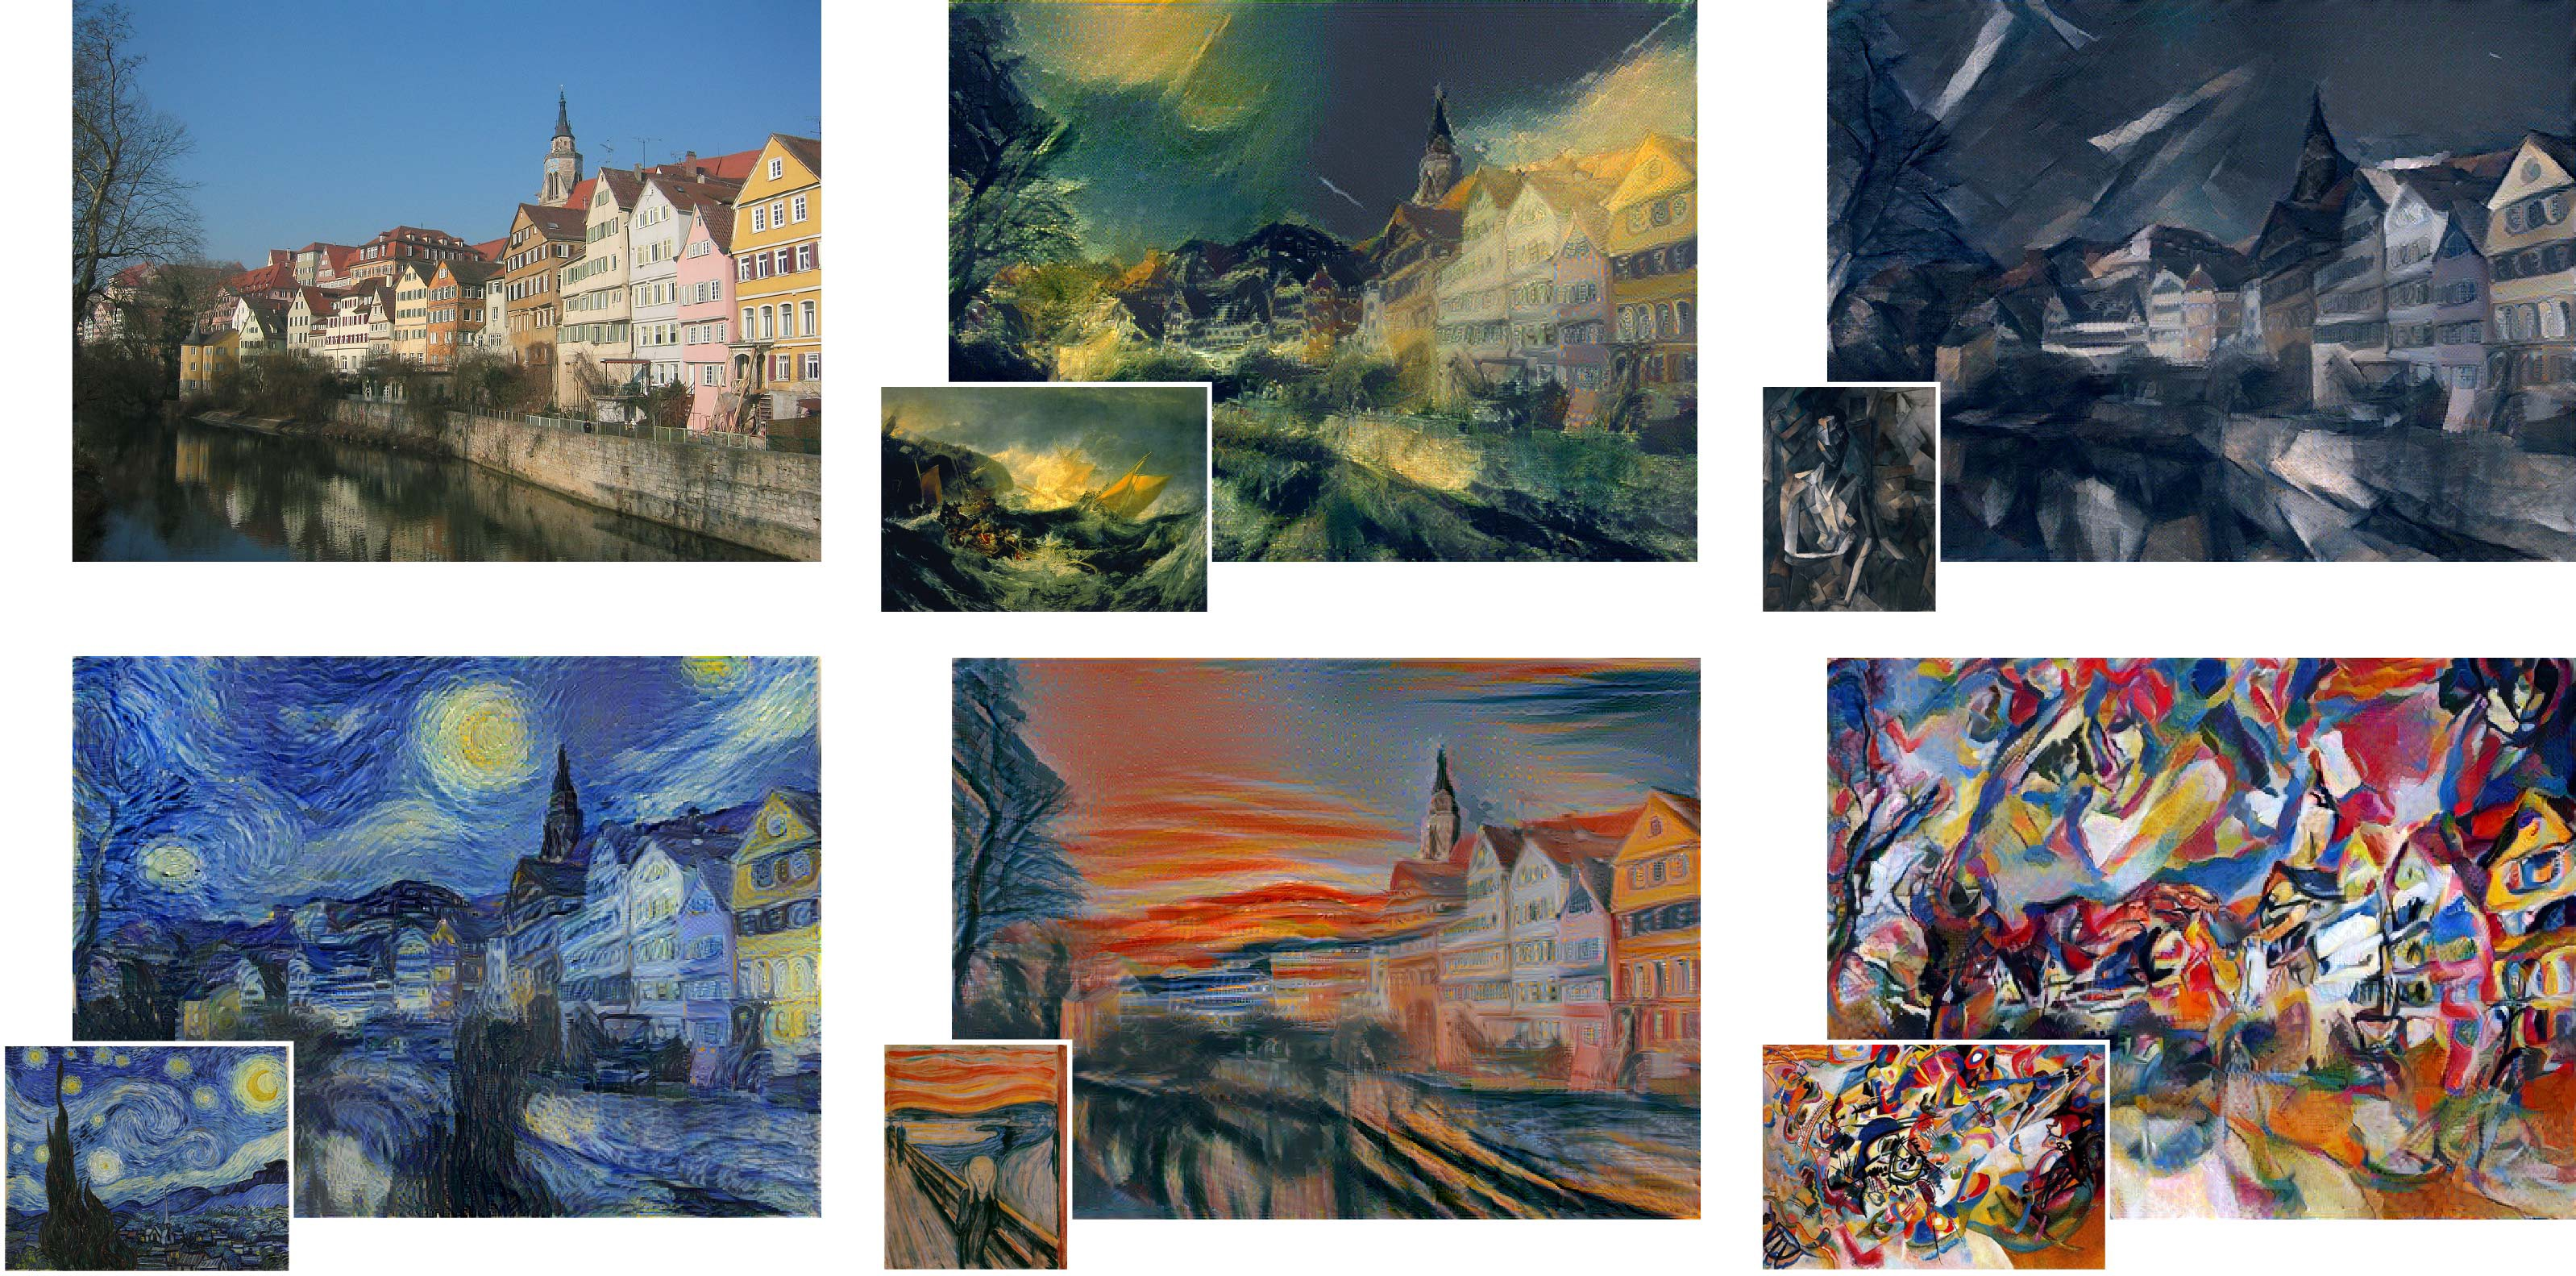
\includegraphics[width=0.9\textwidth]{style-transfer.jpeg}
          \caption{Deep Style Transfer}
          \label{fig:jim_carrey}
        \end{figure}
      \end{column}
    \end{columns}
  \end{frame}

  \begin{frame}
    \frametitle{Deep Learning and What Makes it Interesting}
    \begin{columns}
      \begin{column}{0.5\textwidth}
        \begin{itemize}
          \item Machines making sense of the world; Recognizing patterns
          \item (Pseudo) Artificial neurons, like you have in your brain
          \item We perceive things intuitively, but it is quite difficult for a machine
          \item Deep Learning is a set of cool techniques that can be transfered to many places
          \item State-of-the-art in almost every field it has been applied to
        \end{itemize}
      \end{column}
      \begin{column}{0.5\textwidth}
        \begin{figure}[th!]
          \centering
          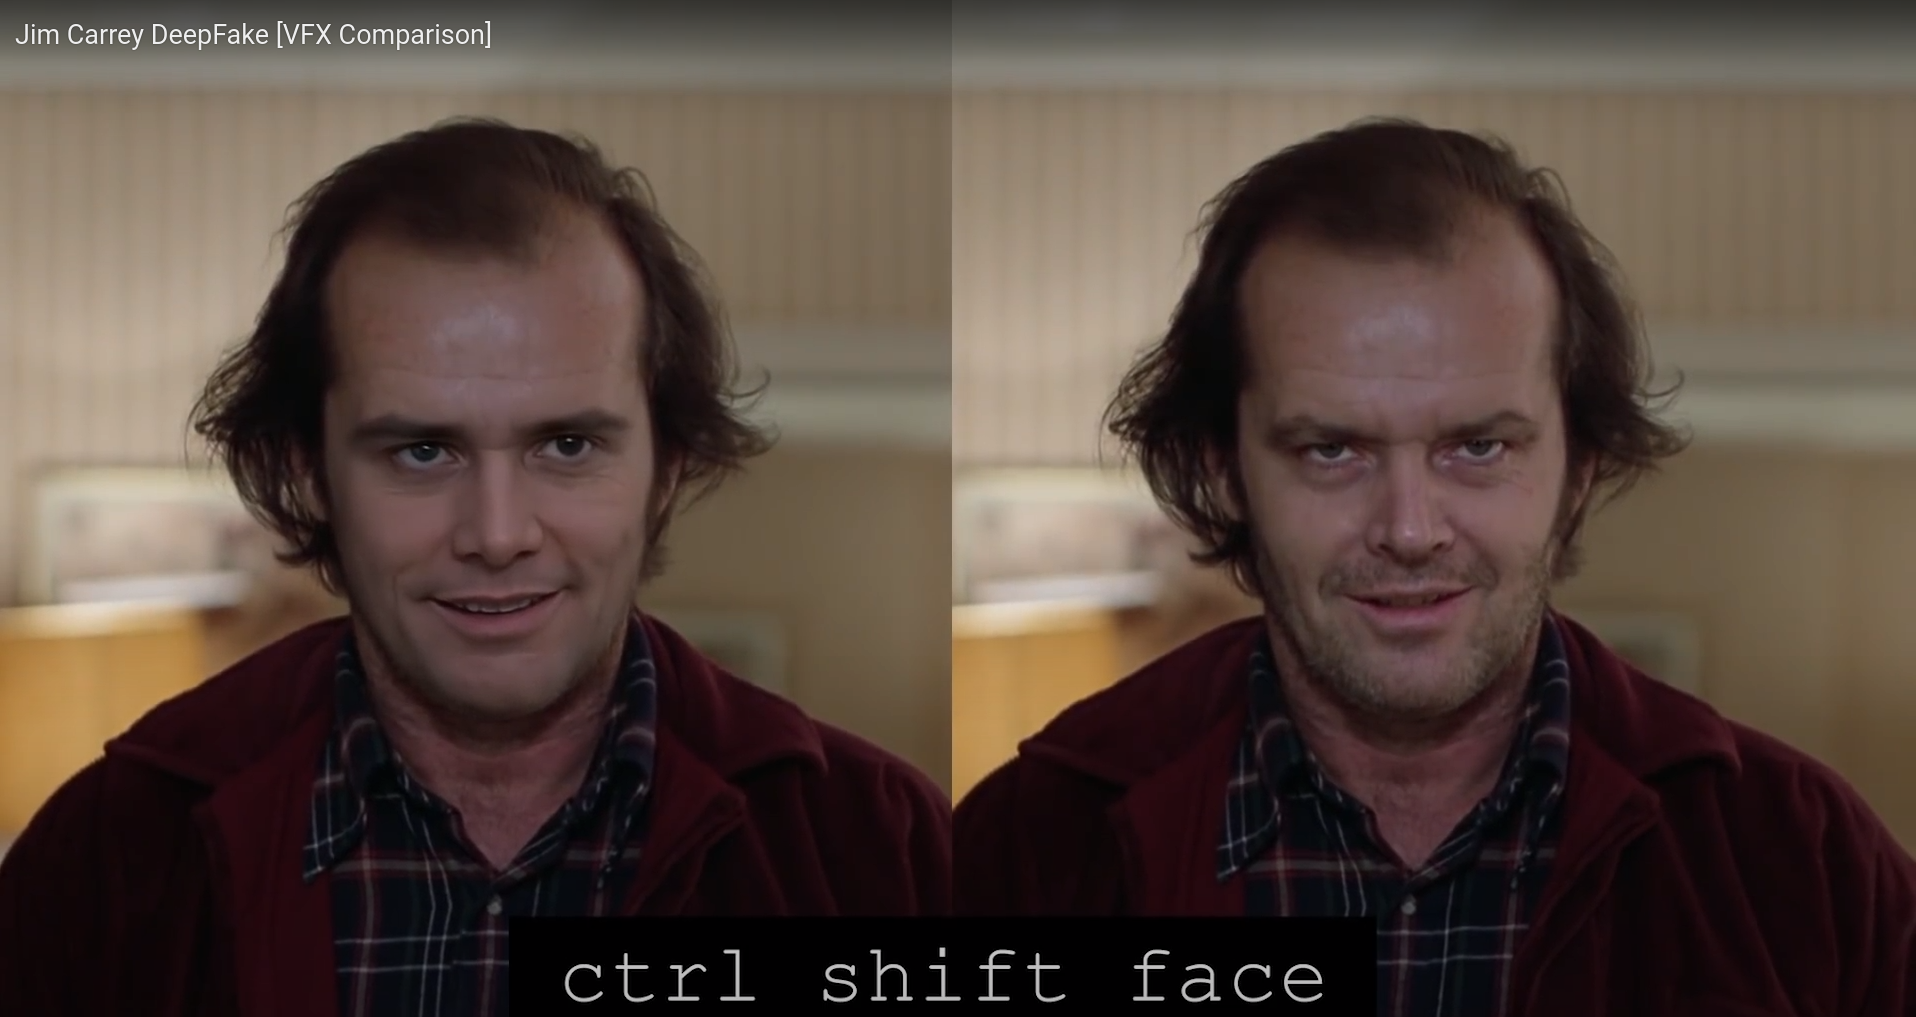
\includegraphics[width=1\textwidth]{jim_carrey.png}
          \caption{Jim Carrey (left) as Jack Nicholson (right), the shining deep fake.\autocite{deepfake}}
          \label{fig:jim_carrey}
        \end{figure}
      \end{column}
    \end{columns}
  \end{frame}

  \begin{frame}
    \frametitle{Thus Our Problem}
    \begin{columns}
      \begin{column}{0.5\textwidth}
        \begin{itemize}
          \item We have this wonderfully whimsical technology
          \item Its incredibly effective at specific tasks
          \item It requires a lot of data to learn
          \item Where do we get this data?
          \item What sort of deep learning, neural networks do we create?
        \end{itemize}
      \end{column}
      \begin{column}{0.5\textwidth}
        \begin{figure}[th!]
          \centering
          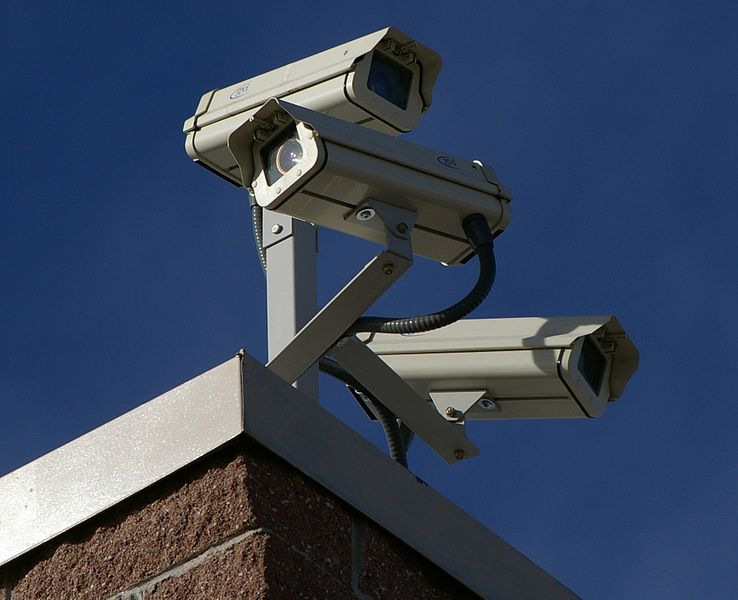
\includegraphics[width=1\textwidth]{surveillance.jpg}
          \caption{Surveillance by Hustvedt \autocite{cc}}
          \label{fig:jim_carrey}
        \end{figure}
      \end{column}
    \end{columns}
  \end{frame}

  \begin{frame}
    \frametitle{Solutions}
    \begin{columns}
      \begin{column}{0.5\textwidth}
        \begin{itemize}
          \item Don't
          \item Federated learning (collaborative distributed models)
          \item Differential privacy (anonymise individuals)
          \item Fully Homomorphic Encryption (compute on encrypted data)
        \end{itemize}
      \end{column}
      \begin{column}{0.5\textwidth}
        \begin{figure}[th!]
          \centering
          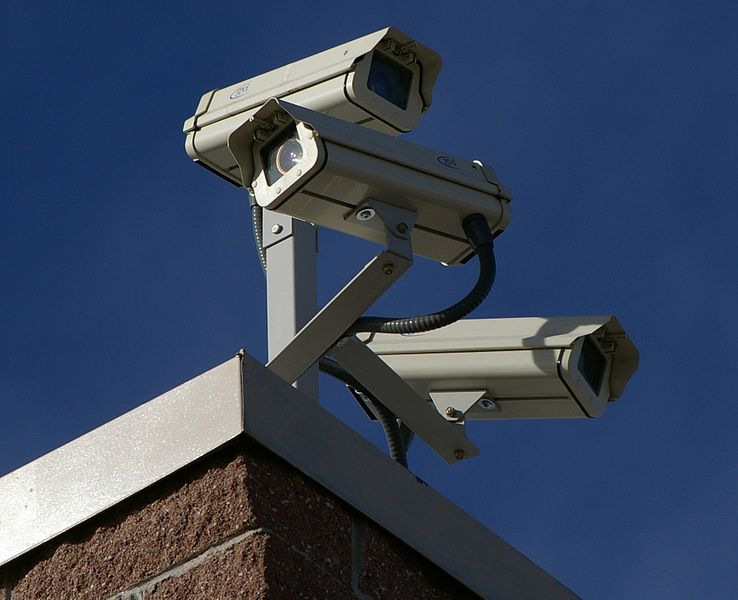
\includegraphics[width=1\textwidth]{surveillance.jpg}
          \caption{Surveillance by Hustvedt \autocite{cc}}
          \label{fig:jim_carrey}
        \end{figure}
      \end{column}
    \end{columns}
  \end{frame}

  \begin{frame}
    \frametitle{Fully Homomorphic Encryption and What Makes it Interesting}
    \begin{columns}
      \begin{column}{0.5\textwidth}
        \begin{itemize}
          \item Allows encrypted data to be added and multiplied with/to
          \item Gives us an alternative to protect sensitive data
          \item Simple operations yet they achieve the otherwise impossible
          \item Use deep learning on something encrypted like diagnosis, and prediction with trade secrets
        \end{itemize}
      \end{column}
      \begin{column}{0.5\textwidth}
        \begin{figure}[th!]
          \centering
          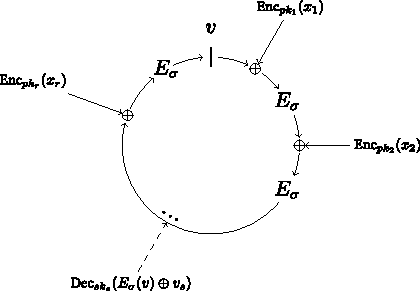
\includegraphics[width=1\textwidth]{ring-signature.pdf}
          \caption{Ring signature, by Chouhartem}
          \label{fig:jim_carrey}
        \end{figure}
      \end{column}
    \end{columns}
  \end{frame}

  \begin{frame}
    \frametitle{Overview of FHE/ CKKS}
    \begin{columns}
      \begin{column}{0.5\textwidth}
        Overview of Cheon, Kim, Kim and Song (CKKS) \autocite{cheon2017homomorphic, cheon2018bootstrapping} FHE scheme:
        \begin{itemize}
          \item Operates on vectors of complex values $\mathbb{C}$, thus useful for floating point operations such as those in deep learning, unlike many other schemes
          \item Encodes complex values as polynomials known as the plaintext
          \item Encrypts plaintext using public key
          \item Cyphertext that addition, multiplication, and rotation can be applied to
          \item Decrypt using private key into plaintext polynomials
          \item Decode plaintext to complex values
        \end{itemize}
      \end{column}
      \begin{column}{0.5\textwidth}
        \begin{figure}[th!]
          \centering
          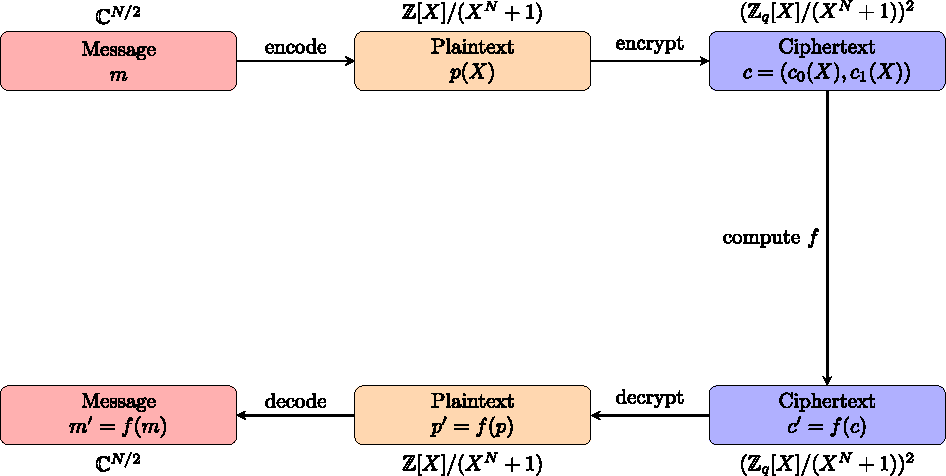
\includegraphics[width=1\textwidth]{fhe-overview.pdf}
          \caption{FHE / CKKS operation overview \autocite{openmined}}
          \label{fig:jim_carrey}
        \end{figure}
      \end{column}
    \end{columns}
  \end{frame}

  \begin{frame}
    \frametitle{Deep Learning on CKKS Cyphertext Example (Point Wise)}
    \begin{columns}
      \begin{column}{1\textwidth}
        \begin{figure}[th!]
          \centering
          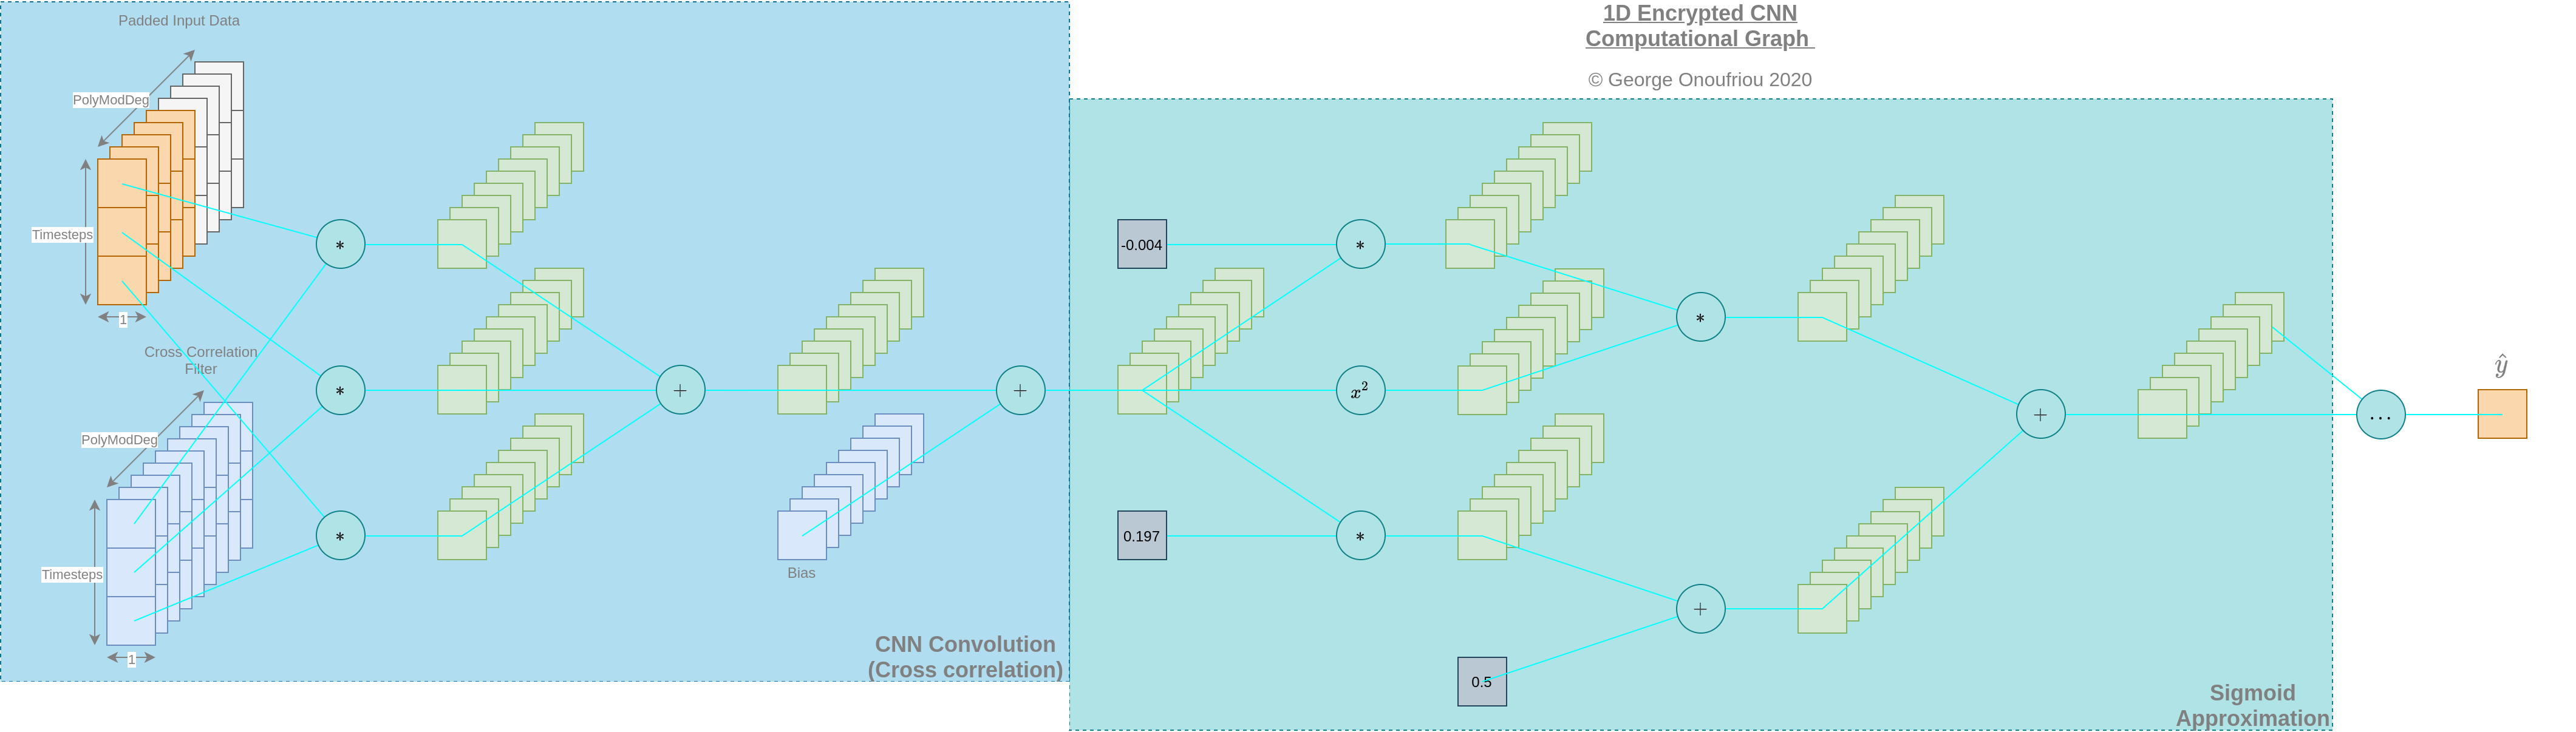
\includegraphics[width=0.9\textwidth]{encrypted_cnn.png}
          \caption{Encrypted convolutional neural network example \autocite{repository}}
          \label{fig:cnn}
        \end{figure}
      \end{column}
    \end{columns}
  \end{frame}

  \begin{frame}
    \frametitle{Deep Learning on CKKS Cyphertext Example (Example Wise)}
    \begin{columns}
      \begin{column}{1\textwidth}
        \begin{figure}[th!]
          \centering
          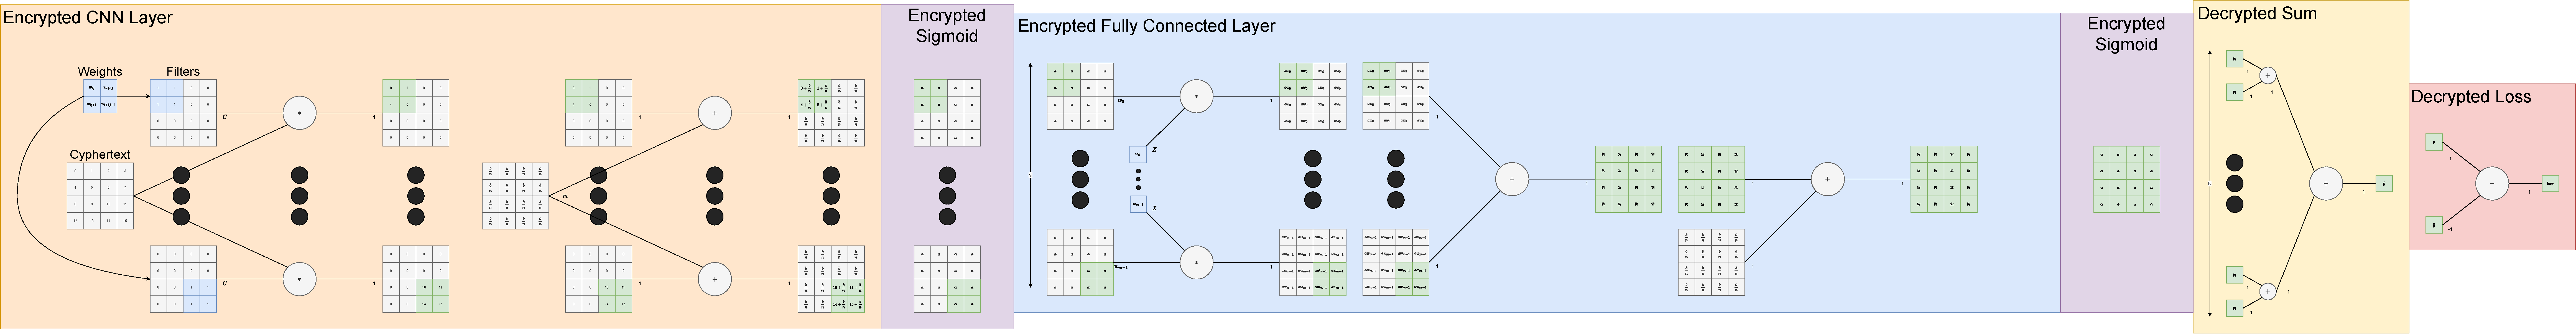
\includegraphics[width=1\textwidth]{example_wise_computational_graph.pdf}
          \caption{Encrypted convolutional neural network example \autocite{repository}}
          \label{fig:cnn}
        \end{figure}
      \end{column}
    \end{columns}
  \end{frame}

  \begin{frame}
    \frametitle{Deep Learning Neuron}
    \begin{columns}
      \begin{column}{0.5\textwidth}
        \begin{figure}[th!]
          \centering
          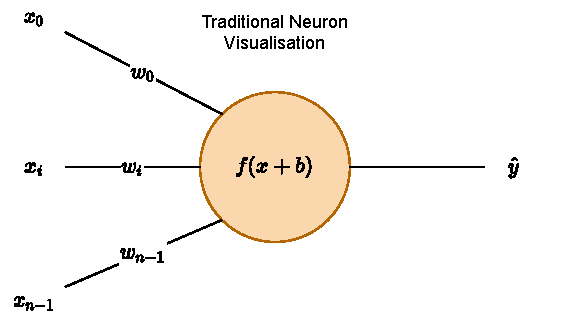
\includegraphics[width=1\textwidth]{neuron.pdf}
          \caption{Articial neural network neuron. \autocite{repository}}
          \label{fig:neuron}
        \end{figure}
      \end{column}
    \end{columns}
  \end{frame}

  \begin{frame}
    \frametitle{Neuron as Computational Graph}
    \begin{columns}
      \begin{column}{0.5\textwidth}
        \begin{figure}[th!]
          \centering
          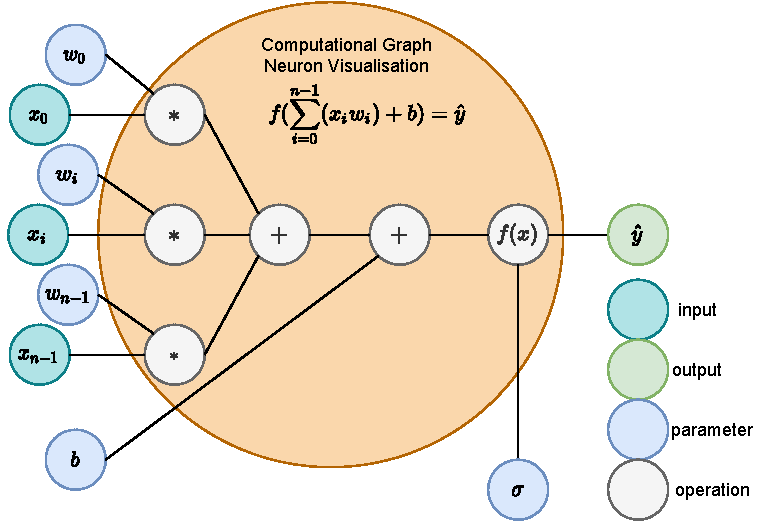
\includegraphics[width=1\textwidth]{neuron_computational_graph.pdf}
          \caption{Articial neural network neuron as computational graph. \autocite{repository}}
          \label{fig:neuron}
        \end{figure}
      \end{column}
    \end{columns}
  \end{frame}

  \begin{frame}
    \frametitle{Activation functions $f$}
    \begin{columns}
      \begin{column}{1\textwidth}
        \begin{figure}[th!]
          \centering
          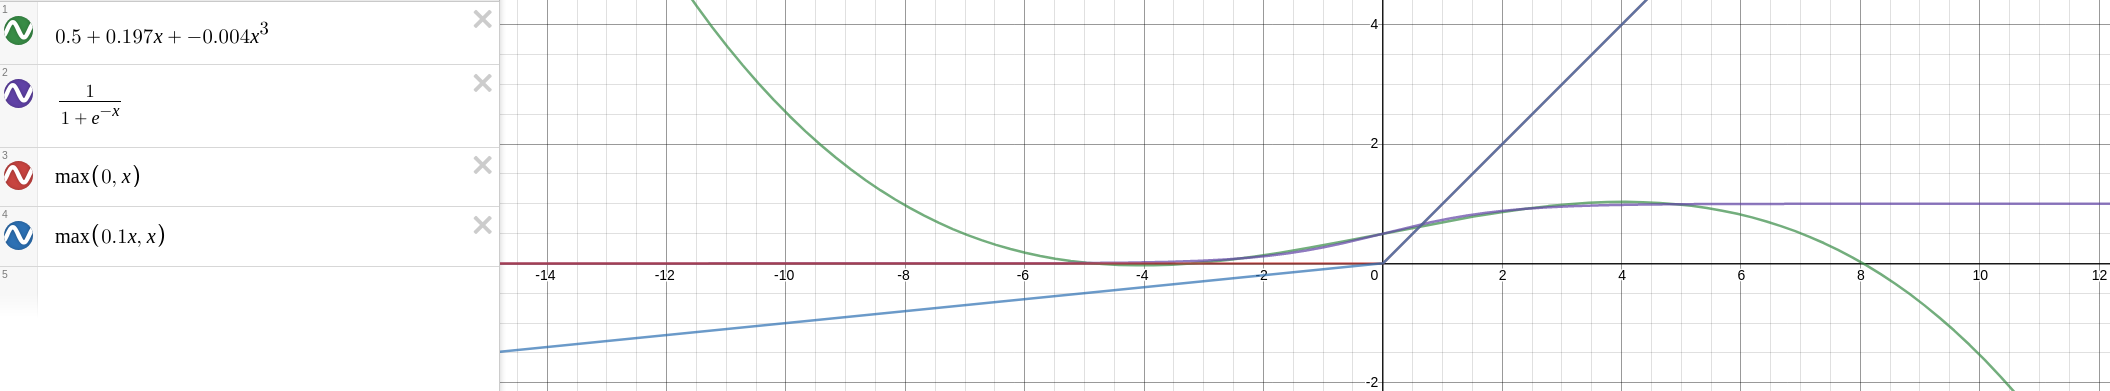
\includegraphics[width=1\textwidth]{activations.png}
          \caption{Articial neural network activation functions; Sigmoid approximation, sigmoid, ReLU, leaky-ReLU. \autocite{repository}}
          \label{fig:approximation}
        \end{figure}
      \end{column}
    \end{columns}
  \end{frame}

  \begin{frame}
    \frametitle{How do we do it specifically}
    \begin{columns}
      \begin{column}{0.5\textwidth}
        To put everything together:
        \begin{itemize}
          \item Aware of computational depth
          \item Whatever we encrypt becomes final
          \item Have to use abelian/ compatible operations only (+, *, +(-x))
        \end{itemize}
      \end{column}
      \begin{column}{0.5\textwidth}
        \begin{figure}[th!]
          \centering
          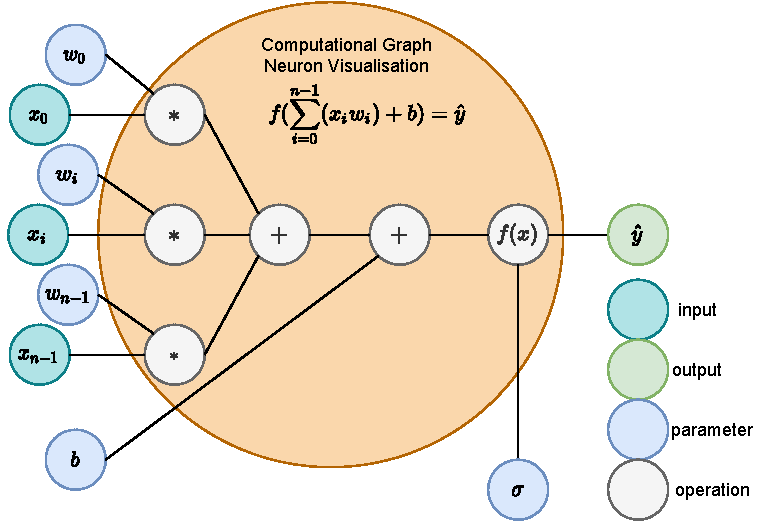
\includegraphics[width=1\textwidth]{neuron_computational_graph.pdf}
          \caption{DL Neuron \autocite{openmined}}
        \end{figure}
      \end{column}
    \end{columns}
  \end{frame}

  \begin{frame}
    \frametitle{CNN as Computational Graph}
    \begin{columns}
      \begin{column}{1\textwidth}
        \begin{figure}[th!]
          \centering
          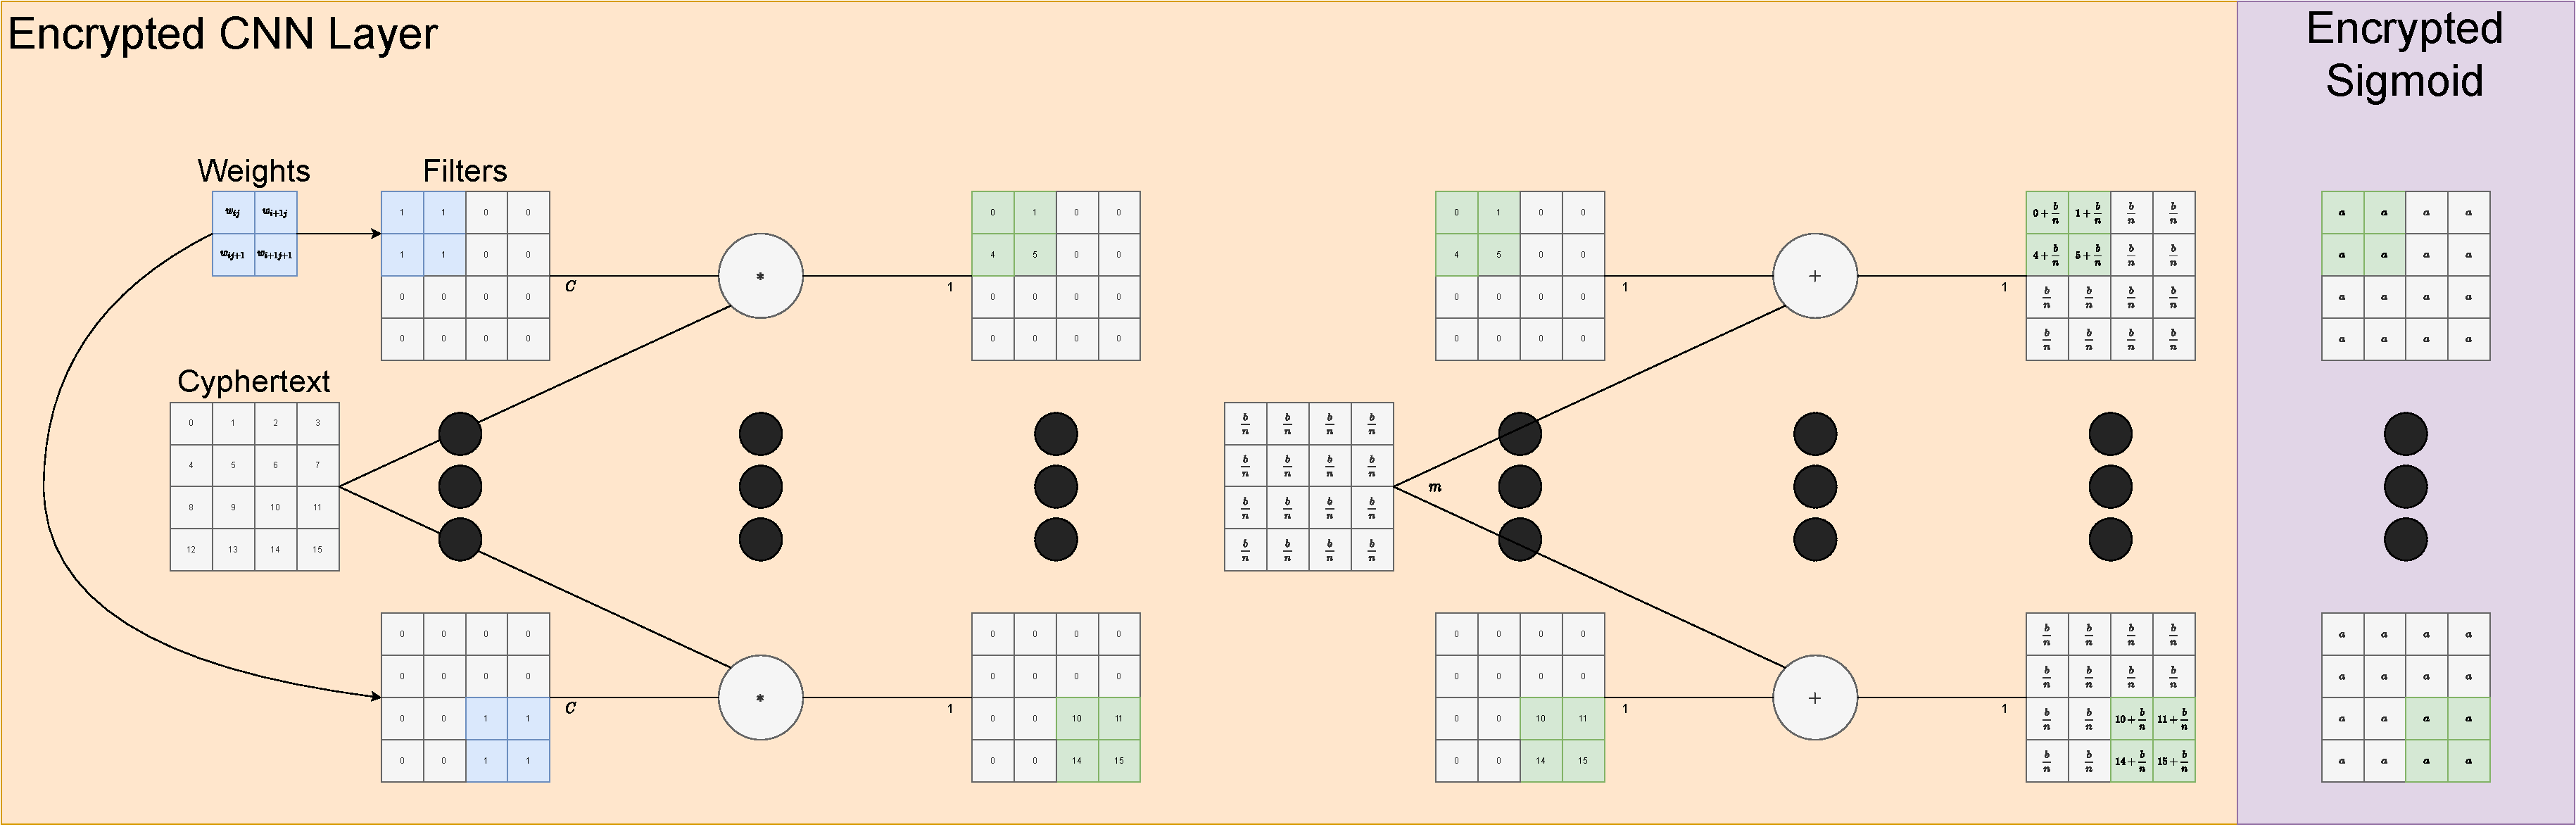
\includegraphics[width=1\textwidth]{cnn_computational_graph.pdf}
          \caption{Convolutional neural network as computational graph. \autocite{repository}}
          \label{fig:cnn_computational_graph}
        \end{figure}
      \end{column}
    \end{columns}
  \end{frame}

  \begin{frame}
    \frametitle{Hadmard Product}
    \begin{columns}
      \begin{column}{1\textwidth}
        \begin{figure}[th!]
          \centering
          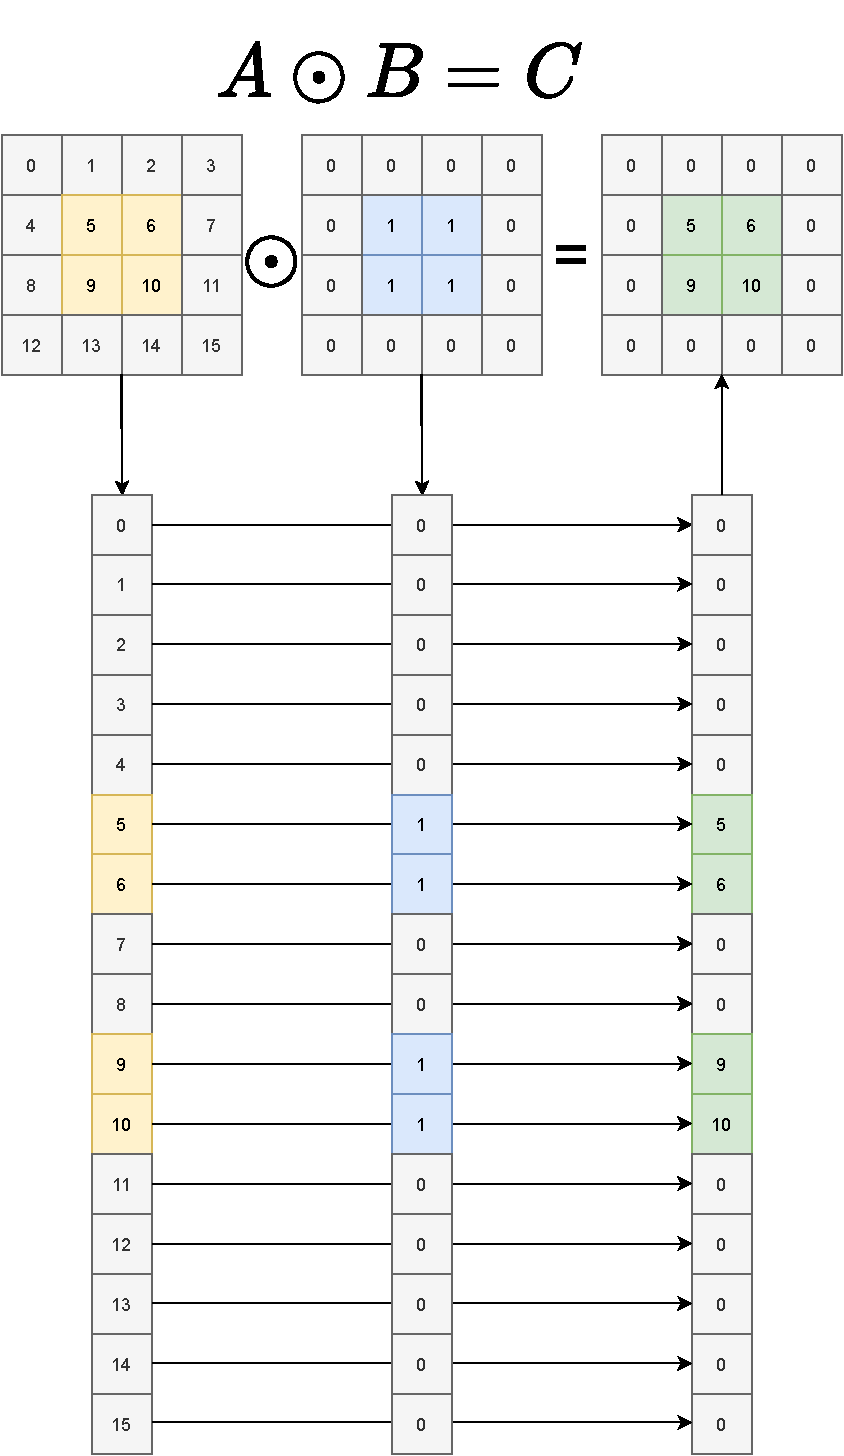
\includegraphics[width=0.25\textwidth]{hadmard_product.pdf}
          \caption{Hadmard Product of two matrices. \autocite{repository}}
          \label{fig:hadmard_product}
        \end{figure}
      \end{column}
    \end{columns}
  \end{frame}

  \begin{frame}
    \frametitle{ANN as Computational Graph}
    \begin{columns}
      \begin{column}{1\textwidth}
        \begin{figure}[th!]
          \centering
          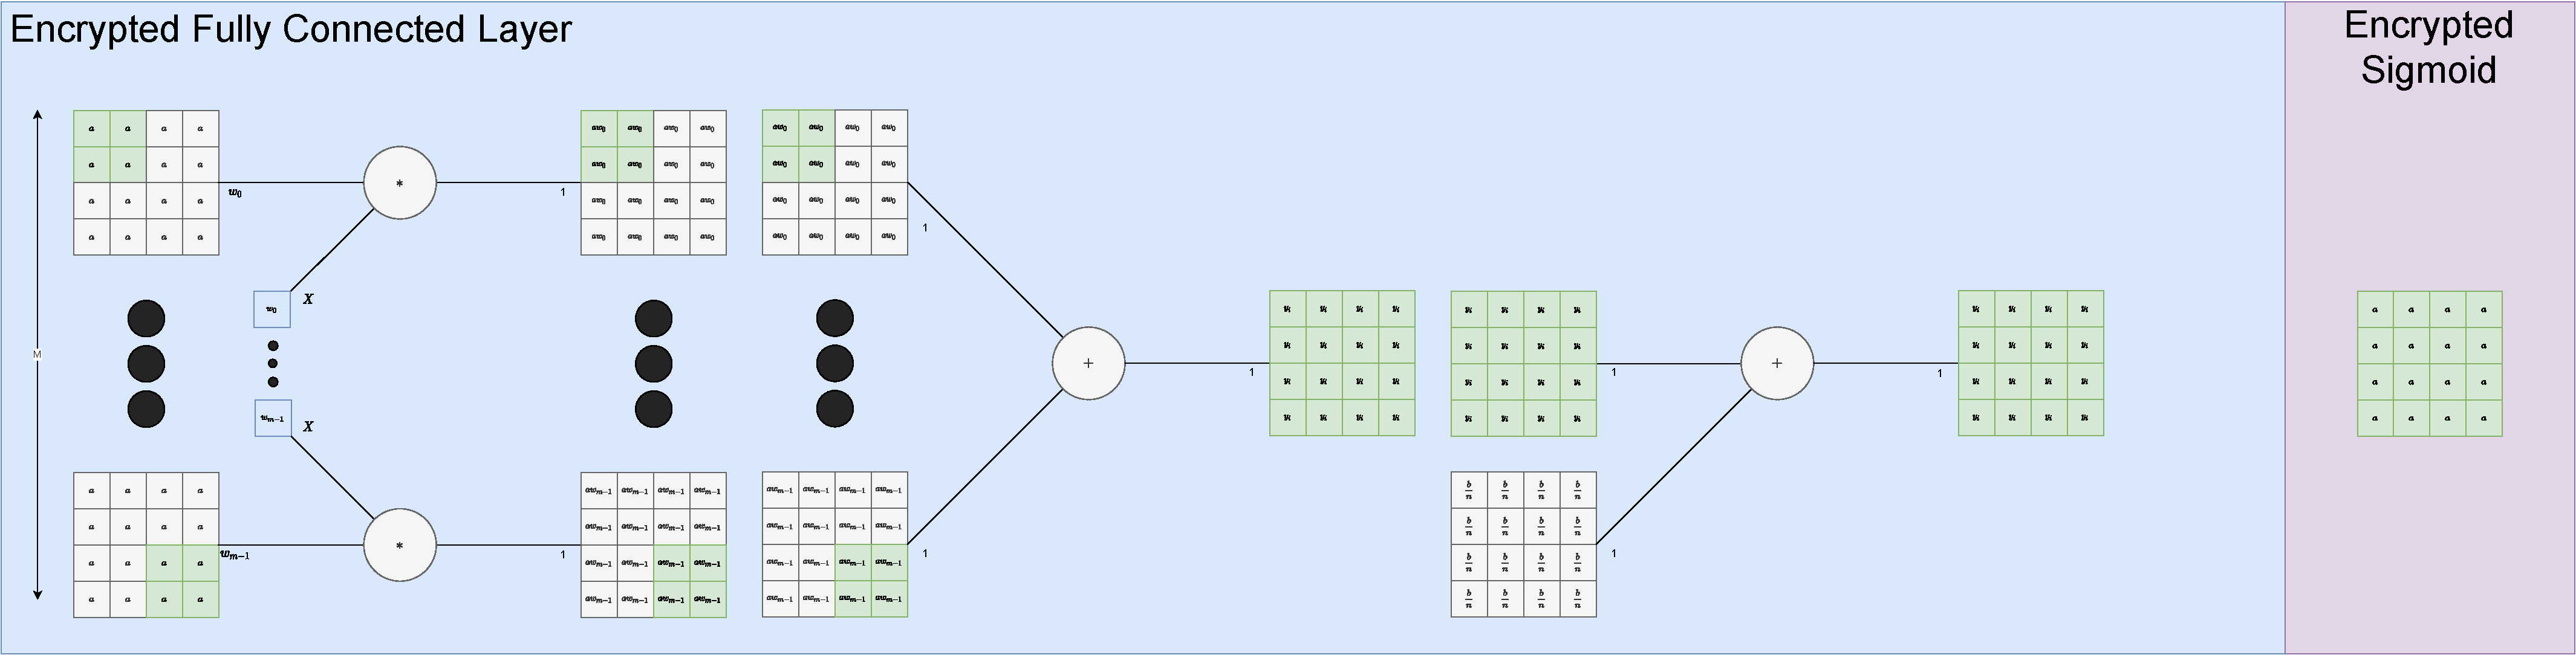
\includegraphics[width=1\textwidth]{dense_computational_graph.pdf}
          \caption{Dense/ ANN neural network as computational graph. \autocite{repository}}
          \label{fig:dense_computational_graph}
        \end{figure}
      \end{column}
    \end{columns}
  \end{frame}

  \begin{frame}
    \frametitle{Loss as Computational Graph}
    \begin{columns}
      \begin{column}{1\textwidth}
        \begin{figure}[th!]
          \centering
          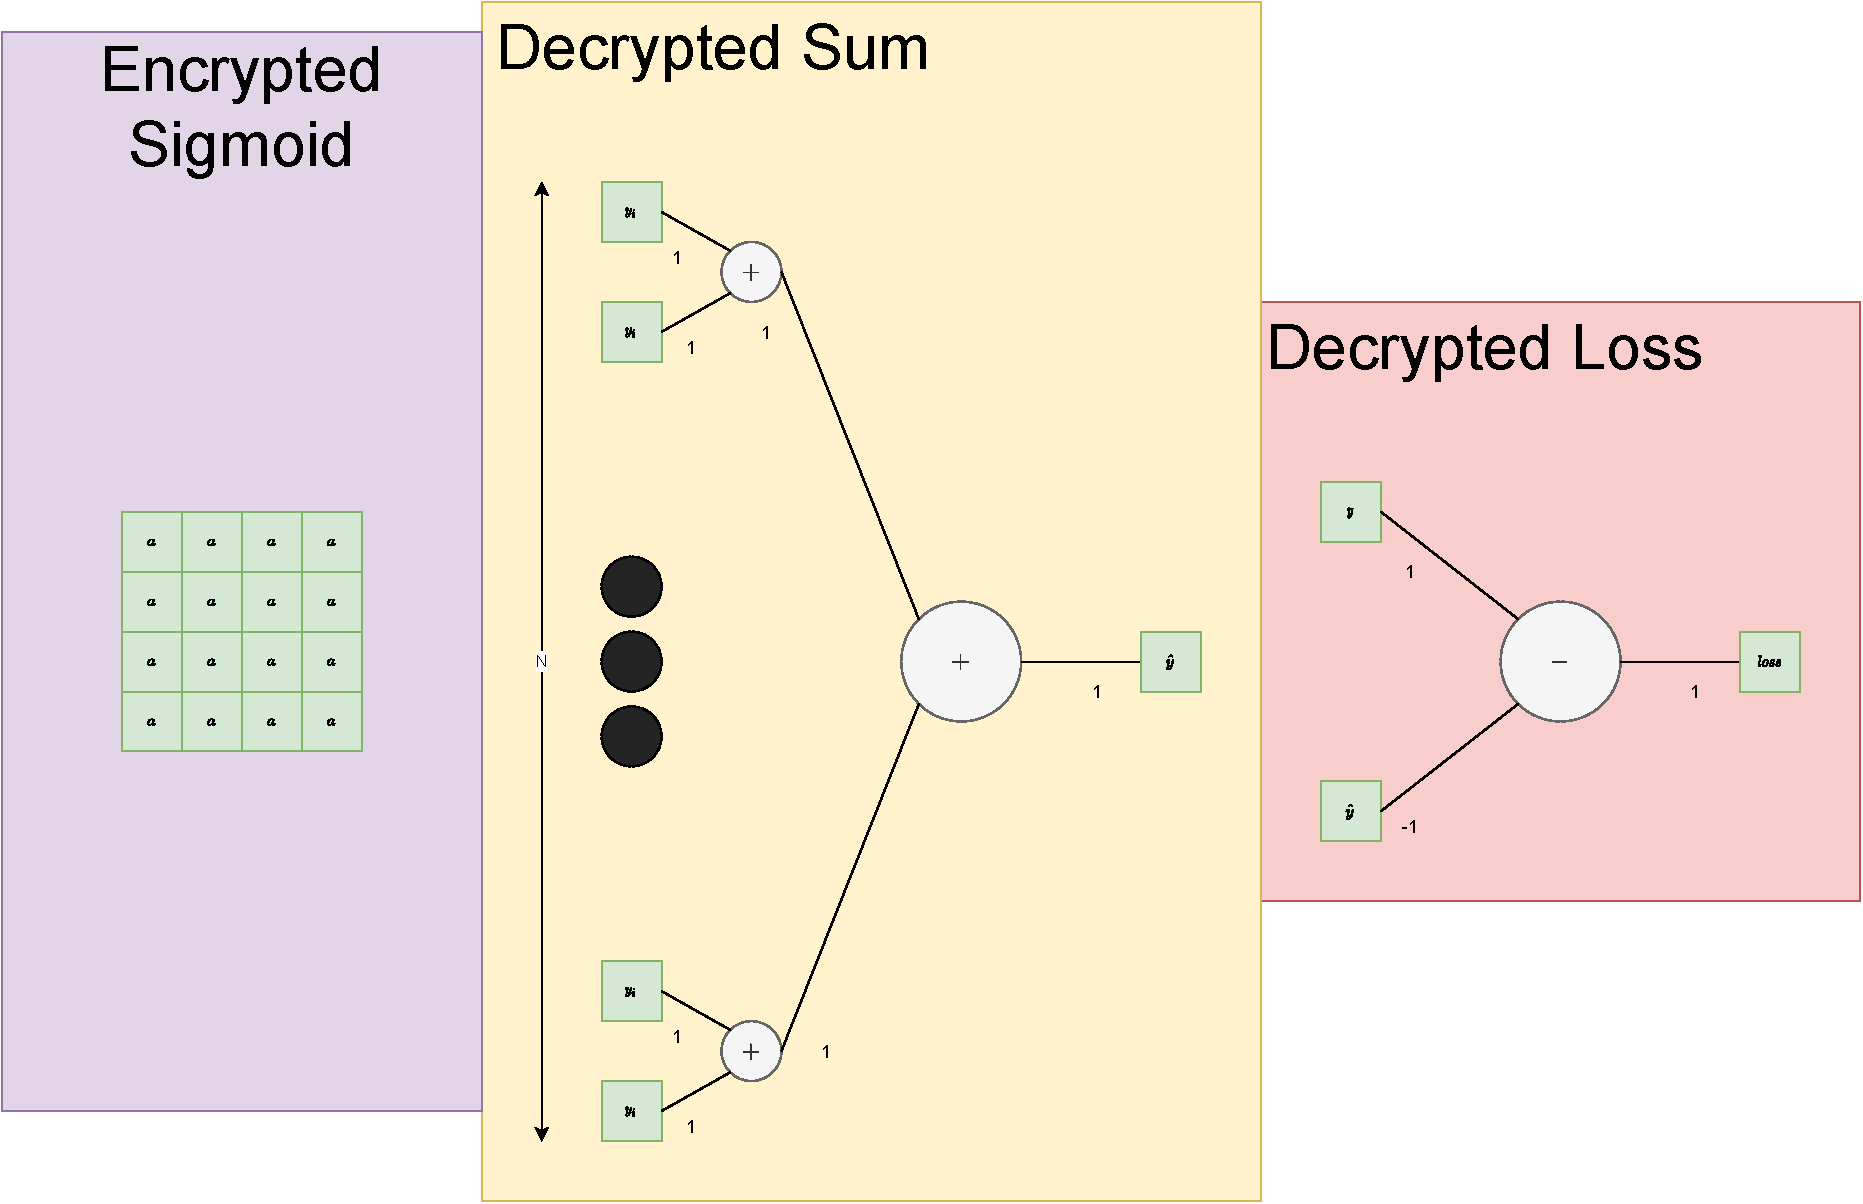
\includegraphics[width=0.7\textwidth]{loss_computational_graph.pdf}
          \caption{Calculating loss/ error of our predictions, our wrongness. \autocite{repository}}
          \label{fig:loss_computational_graph}
        \end{figure}
      \end{column}
    \end{columns}
  \end{frame}

  \begin{frame}
    \frametitle{Alternative Use Computational Graph}
    \begin{columns}
      \begin{column}{0.5\textwidth}
        \begin{figure}[th!]
          \centering
          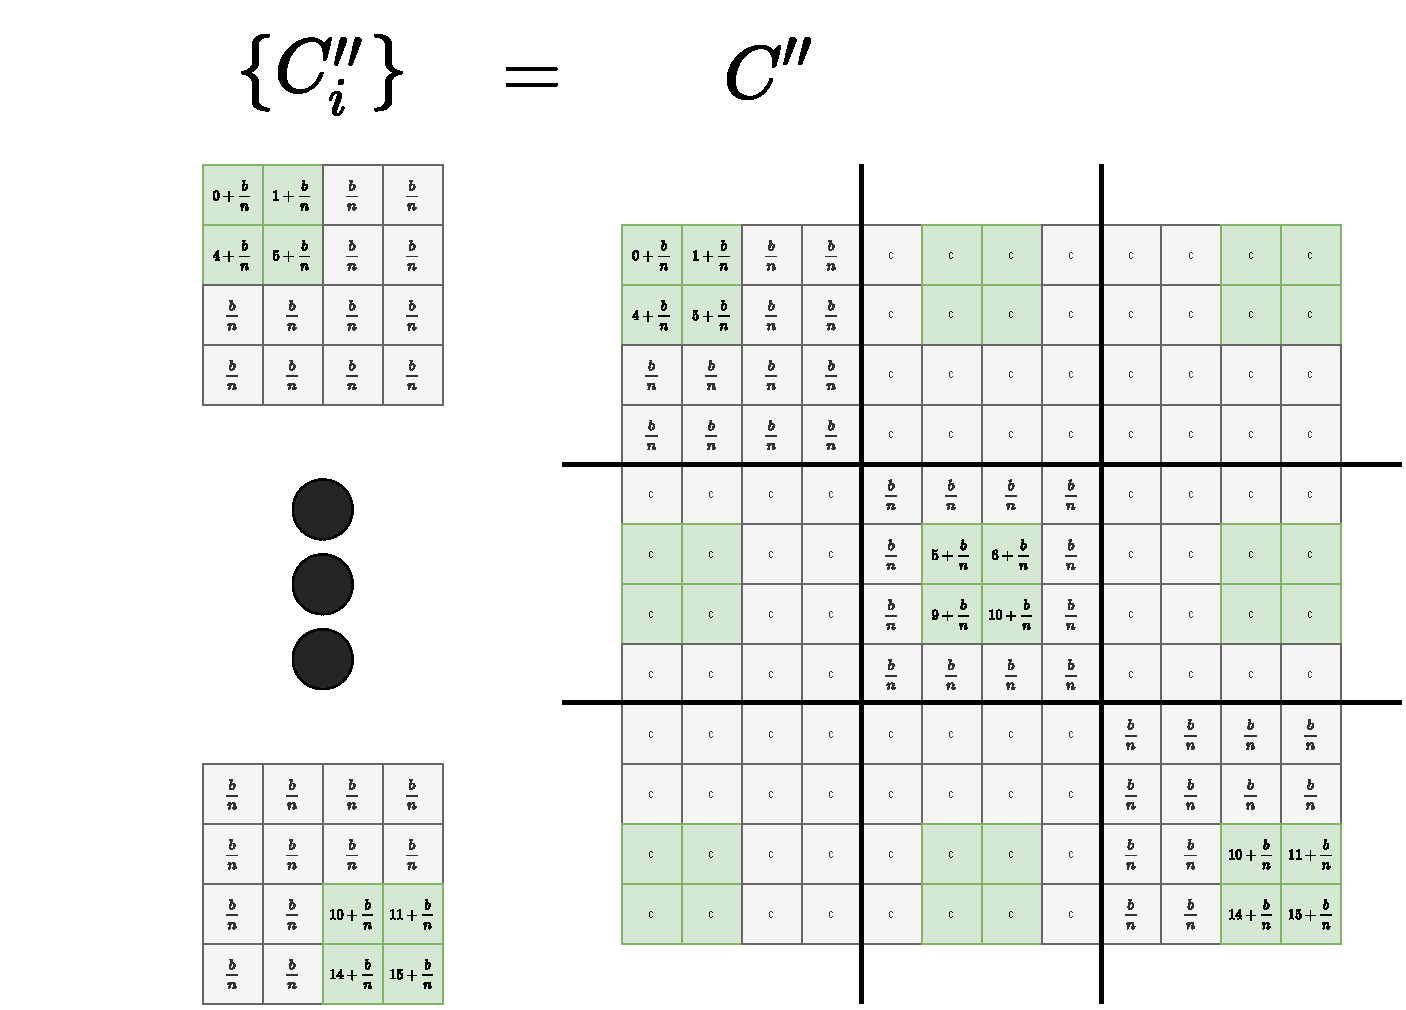
\includegraphics[width=0.7\textwidth]{alternative_computational_graph.pdf}
          \caption{CNN alternatives for multiple deeper layers, for other use cases. \autocite{repository}}
          \label{fig:alternative_computational_graph}
        \end{figure}
      \end{column}
      \begin{column}{0.5\textwidth}
        \begin{figure}[th!]
          \centering
          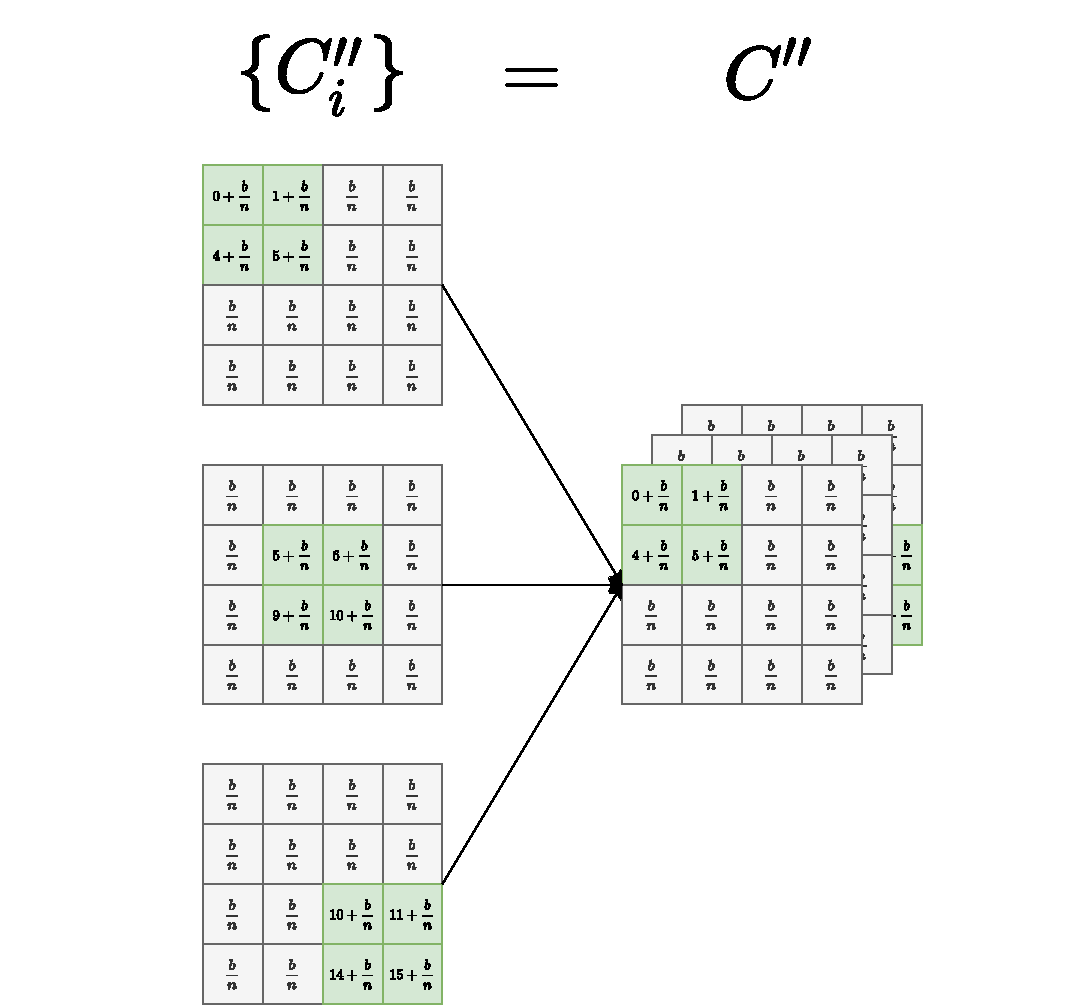
\includegraphics[width=0.7\textwidth]{alternative_computational_graph_2.pdf}
          \caption{CNN alternatives for multiple deeper layers, for other use cases. \autocite{repository}}
          \label{fig:alternative_computational_graph_2}
        \end{figure}
      \end{column}
    \end{columns}
  \end{frame}

  \begin{frame}
    \frametitle{Interested?}
    \begin{columns}
      % \begin{column}{0.5\textwidth}
      %   I got here through textbook approach:
      %   \begin{itemize}
      %     \item A-Levels (Sciences)
      %     \item BSc Computer Science
      %     \item PhD Computer Science
      %   \end{itemize}
      %   Computer Science takes you places, as it is so broad.\\
      %   Everyone is different you might go a different route:
      %   \begin{itemize}
      %     \item Computer science can be learned easily by anyone with a reasonable computer and internet connection for free
      %   \end{itemize}
      % \end{column}
      \begin{column}{0.5\textwidth}
        Good places to start are:
        \begin{itemize}
            \item Deep Learning by Goodfellow et al \autocite{Goodfellow-et-al-2016}
            \item Coursera deep learning specialisation
            \item Andrej Karpathy's youtube series on deep learning \autocite{andrejkarpathy}
            \item CKKS explained (OpenMined) \autocite{openmined}
        \end{itemize}
      \end{column}
      \begin{column}{0.5\textwidth}
        There are relativeley few practical implementations that will work (support CKKS, serialisable, bootstrapping):
        \begin{itemize}
            \item our own library (and soon to be docs): \url{https://github.com/DreamingRaven/python-reseal} 
        \end{itemize}
      \end{column}
    \end{columns}
  \end{frame}

  \begin{frame}
    \frametitle{Summary}
    \begin{columns}
      \begin{column}{0.5\textwidth}
        \begin{itemize}
          \item Introduce myself
          \item Introduce the problem of secrets
          \item What is deep learning
          \item What is fully homomorphic encryption
          \item A rough idea of how it operates
          \item How I got here
          \item How to find out more if it interests you
        \end{itemize}
      \end{column}
      \begin{column}{0.5\textwidth}
        \begin{figure}[th!]
          \centering
          \includegraphics[angle=-90,origin=c,width=0.6\textwidth]{strawberry.jpg}
          \caption{A strawberry for your time. \autocite{repository}}
          \label{fig:strawberry}
        \end{figure}
      \end{column}
    \end{columns}
  \end{frame}

  \begin{frame}[allowframebreaks]
    \frametitle{References}
    % % biblatex version
    \printbibliography
  \end{frame}

  \begin{frame}
      \frametitle{Questions}
      Come and ask questions!
      \url{https://github.com/DreamingRaven/encrypted-deep-learning-presentation}
  \end{frame}


\end{document}
